\documentclass[11pt]{article}
% Shared preamble for main.tex and the appendix files.
\usepackage[utf8]{inputenc}
\usepackage[T1]{fontenc}
\usepackage{lmodern}
\usepackage{amsmath,amssymb,amsthm,mathtools}
\usepackage{graphicx}
\usepackage{booktabs}
\usepackage{enumitem}
\usepackage[margin=1in]{geometry}
\usepackage[colorlinks=true,linkcolor=blue,citecolor=blue,urlcolor=blue]{hyperref}

\newtheorem{lemma}{Lemma}[section]
\newtheorem{theorem}[lemma]{Theorem}
% Named main results (Theorem A, Corollary 1', ...): unnumbered, with fixed names.
\newtheorem*{thmA}{Theorem A (strict plank bound)}
\newtheorem*{thmB}{Theorem B (constructions)}
\newtheorem*{corC}{Corollary C}
\newtheorem*{thmD}{Theorem D (small $n$)}
\newtheorem*{corOne}{Corollary 1 (Bang is never attained)}
\newtheorem*{corTwo}{Corollary 2 (restricted additive $2$-bases)}
\newtheorem{proposition}[lemma]{Proposition}
\newtheorem{corollary}[lemma]{Corollary}
\newtheorem{claim}[lemma]{Claim}
\theoremstyle{definition}
\newtheorem{definition}[lemma]{Definition}
\theoremstyle{remark}
\newtheorem{remark}[lemma]{Remark}

\numberwithin{equation}{section}
\newcommand{\R}{\mathbb{R}}
\newcommand{\Z}{\mathbb{Z}}
\newcommand{\Q}{\mathbb{Q}}
\newcommand{\N}{\mathbb{N}}
\newcommand{\E}{\mathbb{E}}
\renewcommand{\Pr}{\mathbb{P}}
\newcommand{\ball}{B}                 % \ball^d = closed unit ball
\newcommand{\Sph}{S}                  % \Sph^{d-1} = unit sphere
\newcommand{\eps}{\varepsilon}
\newcommand{\abs}[1]{\left|#1\right|}
\newcommand{\norm}[1]{\left\|#1\right\|}
\newcommand{\ip}[2]{\langle #1,#2\rangle}
\DeclareMathOperator{\dist}{dist}
\DeclareMathOperator{\Var}{Var}
\DeclareMathOperator{\lcm}{lcm}
\DeclareMathOperator{\area}{area}
\DeclareMathOperator{\vol}{vol}
\DeclareMathOperator{\spn}{span}
\DeclareMathOperator{\adj}{adj}

\setlength{\emergencystretch}{1em}

% Local notation for Section 3 (formerly Appendix A).
\newcommand{\Abb}{\bar\beta}
\newcommand{\AH}{\mathcal{H}}
\newcommand{\AI}{\mathcal{I}}
\newcommand{\Aone}{\mathbf{1}}
\newcommand{\Adep}{\#\mathrm{dep}}

\title{Planks through points: covering a ball by slabs\\ around spanned hyperplanes}
\author{Michael Werman}
\date{}

\begin{document}
\maketitle

\begin{abstract}
For $n$ points in the unit ball $\ball^d$, let $\rho$ be the smallest $\eps$ such that the $\eps$-slabs around the
hyperplanes spanned by $d$ of the points cover the ball, and let $\lambda_d(n)$ be the infimum of $\rho$. Bang's
plank theorem gives $\binom nd\lambda_d(n)\ge1$, with equality for freely placed hyperplanes. We show that spanned
hyperplanes never attain this bound and lose a constant factor in every dimension:
$\liminf n^d\lambda_d(n)\ge d!\,(1+q_d)$ with an explicit $q_d\ge0.08/\sqrt{d-2}$, and
$\liminf n^2\lambda_2(n)\ge6864/3161\approx2.1715$ in the plane. Conversely, clusters whose hyperplane directions
are sums of angles from restricted additive bases of cyclic groups give $\lambda_d(n)=\Theta(n^{-d})$, with
$\limsup n^2\lambda_2(n)\le9\pi/7$. As a by-product, $n$-element sets whose sums of two distinct elements cover a
cyclic group of order $(7/18-o(1))n^2$ exist, improving the published constants $5/18$ and $1/3$. We also treat
small $n$ in the plane, with one computer-assisted step, and variants for great hyperspheres, points anywhere,
flats and convex bodies.
\end{abstract}

\section{Introduction}\label{sec:intro}

Tarski asked, in 1932, whether planks (slabs between two parallel hyperplanes) covering a convex body must
have total width at least the minimal width of the body \cite{Tarski}; Bang proved that they must \cite{Bang},
and Ball proved the analogous statement for symmetric bodies with widths measured relative to the body
\cite{Ball}. Verreault's survey \cite{Verreault} describes the many variants since. For the unit ball
$\ball^d$, Bang's theorem says that if the slabs of half-width $\eps$ around $k$ hyperplanes cover the ball, then
$\eps\ge1/k$, with equality for $k$ parallel, equally spaced hyperplanes. When the hyperplanes are required to pass
through the centre, the answer is $\sin(\pi/2k)$, attained by $k$ hyperplanes through a common $(d-2)$-flat at successive angles
$\pi/k$: this is Fejes T\'oth's zone conjecture, proved by Jiang and Polyanskii \cite{JP} (see also
Zhao \cite{Zhao}).

We ask how well the hyperplanes can cover when they are spanned by a set of points. Let $P$ be a set of $n$
points in $\ball^d$, let $\rho(P)$ be the covering radius of the hyperplanes spanned by $d$ of them, and let
$\lambda_d(n)$ be the infimum of $\rho(P)$ (Section~\ref{sec:results}). There are at most $K=\binom nd$ such
hyperplanes, so Bang's theorem gives $\lambda_d(n)\ge1/K$, and the question is whether spanned hyperplanes can be as
efficient as free ones. They cannot be parallel, since every point of $P$ lies on many of them, and they cannot all
pass through a common $(d-2)$-flat at the centre either, unless the points cluster there.

\paragraph{Results.} Theorem~A shows that spanned hyperplanes lose a constant factor in every dimension:
$\liminf n^d\lambda_d(n)\ge d!\,(1+q_d)$ with $q_2=1/15$, $q_3=1/12$ and $q_d\ge0.08/\sqrt{d-2}$, and sharper
constants $6864/3161\approx2.1715$ in the plane and $20/3$ in space (Section~\ref{sec:A-sharp}); and
Corollary~1 shows that Bang's bound is never attained for $n>d$. The proof integrates the quadratic test function
$(t-m_0)^2$ of the height against a measure whose height is uniform, built from $2$-dimensional great spheres
of random $3$-dimensional sections, and plays the mass that steep slabs carry against the tilt that Bang's sign
argument allows them.

For upper bounds, Theorem~B builds clusters near the centre whose hyperplanes pass close to a common
$(d-2)$-flat, with directions given by sums of $d$ distinct elements of a set in a cyclic group $\Z_N$. So
$\lambda_d(n)\le\sin(\pi/2p_d(n))$, where $p_d(n)$ is the largest $N$ for which some $n$-subset of $\Z_N$ has every
residue as such a sum, and a blow-up construction shows that $\sigma_d=\lim p_d(n)/n^d$ exists and equals
$\sup p_d(n)/n^d$. Hence $\lambda_d(n)=\Theta(n^{-d})$ (Corollary~C), and in the plane
$\limsup n^2\lambda_2(n)\le9\pi/7$, using a $12$-element set in $\Z_{56}$ from Haanp\"a\"a's tables \cite{Haanpaa}.
The same blow-up gives Corollary~2: $p_2(n)\ge(7/18-o(1))n^2$. To our knowledge the best published constants for
this largest-modulus problem were $5/18$, for sums of two distinct elements (Graham and Sloane \cite{GS}), and
$1/3$, for sums of at most two elements (Jia and Shen \cite{JS}; see also \cite[Section~B.1]{Bajnok}).

For small $n$ in the plane, Theorem~D shows that the centred square ($n=4$) and the regular hexagon ($n=6$) beat
every cluster shrinking to the centre. For $n=6$ this rests on a computer-assisted lower bound for $\gamma_6$, the
smallest possible largest gap between the directions of the lines spanned by six points; Appendix~\ref{app:cert}
describes the exact branch-and-bound behind it. This is the only computer-assisted step in the paper.

Section~\ref{sec:ext} treats variants: great hyperspheres through points of the sphere, points placed anywhere in
$\R^d$, the flats spanned by $j+1$ points, and general convex bodies. In a companion paper \cite{Companion} we treat
random points: for $n$ independent uniform points in a convex body $\Omega\subset\R^d$, $n^d\rho/\log n$ converges in
probability to an explicit constant.

\paragraph{Related work.} The quantity $\sin(\gamma_n/2)$ appears as $\rho_2(n)$ in Frankl and Maehara's work on
projecting finite point sets \cite{FM}; we have seen only its zbMATH review, as the full text is not available
online. The sequence $p_2(n)$ is A004131 in the OEIS \cite{OEIS}, which cites their paper, so they may already have
used the link between chord directions and sums in cyclic groups that underlies Theorem~B for $d=2$. We therefore
claim this link as new only for $d\ge3$.

\paragraph{Organisation.} Section~\ref{sec:results} fixes notation and states the results.
Section~\ref{sec:lower} proves the lower bounds, Section~\ref{sec:upper} the constructions and the bounds
on $p_d(n)$, Section~\ref{sec:small} the results for clusters and small $n$, and Section~\ref{sec:ext} the
extensions; Section~\ref{sec:open} lists open problems. Appendix~\ref{app:cert} describes the certified bounds on
$\gamma_5$ and $\gamma_6$, and Appendix~\ref{sec:B-examples} lists the additive-basis examples behind
Table~\ref{tab:bounds}.

\section{Notation and results}\label{sec:results}

For $P\subset\ball^d$ with $|P|=n$, let $\mathcal H_P$ be the set of hyperplanes through $d$ affinely
independent points of $P$, and
\[
K=\binom nd,\qquad \rho(P)=\max_{x\in \ball^d}\,\min_{H\in\mathcal H_P}\dist(x,H),\qquad
\lambda_d(n)=\inf_{|P|=n}\rho(P).
\]
Here $\rho(P)=\infty$ if $P$ has no $d$ affinely independent points, and $n\ge d$ throughout. Several
$d$-subsets may span the same hyperplane, and dependent $d$-subsets span none, so $\mathcal H_P$ has
$K'\le K$ elements; the proofs write $N_H\ge1$ for the number of independent $d$-subsets lying in
$H\in\mathcal H_P$.
For a finite list of hyperplanes $H_j=\{\ip{x}{u_j}=m_j\}$ ($|u_j|=1$), its \emph{covering radius} is
$\max_{x\in\ball^d}\min_j\dist(x,H_j)$; it depends only on the set of hyperplanes.


\begin{thmA}
For $d\ge2$ and $n\ge d$, every $n$-point set $P\subset\ball^d$, with $\rho=\rho(P)$, satisfies
\[
\binom nd\,\rho\ \ge\ \frac{1+q_d}{1+2\rho/A_d},\qquad A_d=\frac{3d-1}{d-1},\qquad
q_d=\min_{|m|\le1}\frac{1/3+m^2}{\Lambda_d(m)},
\]
where $\Lambda_2=A_2$ and, for $d\ge3$,
$\Lambda_d(m)=A_d+(1+|m|)^2(C_d-1)+4(1+|m|)\tfrac{d-3}{d-1}$
with $C_d=\sqrt\pi\,\Gamma(\tfrac{d-1}2)/\Gamma(\tfrac{d-2}2)$; since $C_3=1$, $\Lambda_3=A_3$.
\end{thmA}

So $q_2=1/15$ and $q_3=1/12$, and the bound reads $\binom n2\rho\ge 16/(15+6\rho)$ in the plane and
$\binom n3\rho\ge 13/(12+6\rho)$ in space; for $d\ge4$, $q_d\ge0.08/\sqrt{d-2}$, by hand: exact values of
$C_d$ for $4\le d\le7$, and for $d\ge8$ one quadratic in $m$ with negative discriminant, using
$C_d\le\sqrt{\pi(d-2)/2}$ (Section~\ref{sec:A-qd}). So
$\liminf n^d\lambda_d(n)\ge L_d:=d!\,(1+q_d)$, with $L_2=32/15$, $L_3=13/2$, $L_4\ge25.41$ and
$L_5\ge125.95$. For $d=2,3$ the exact position of the points on their hyperplanes gives larger limit constants:
$\binom n3\rho\ge70/(63+60\rho)$, so $\liminf n^3\lambda_3(n)\ge20/3$, and
$\liminf n^2\lambda_2(n)\ge6864/3161>2.1714$. Complete proofs are in Section~\ref{sec:lower}; the sharper
constants are in Section~\ref{sec:A-sharp}.

\begin{corOne}
$\lambda_d(n)>1/\binom nd$ for every $d\ge2$ and $n>d$.
\end{corOne}

Theorem~A makes this quantitative once $\binom nd>2/(q_dA_d)$: then
\[
\lambda_d(n)\ge\frac{A_d}{4}\Bigl(\sqrt{1+8(1+q_d)\big/\bigl(A_d\tbinom nd\bigr)}-1\Bigr)>1\Big/\tbinom nd.
\]

\begin{thmB}
For $n\ge d+1$, $\lambda_d(n)\le\sin(\pi/2p_d(n))$, where $p_d(n)$ is the largest $N$ such that some
$n$-subset of $\Z_N$ has every residue as a sum of $d$ distinct elements; $n\le p_d(n)\le\binom nd$.
More generally, $\lambda_d(n)\le\sin(G/2)$ whenever $G$ is the largest gap mod $\pi$ of the sums of $d$
distinct elements of some $n$ distinct $\theta$'s in $(0,\pi)$. Moreover,
$\sigma_d=\lim p_d(n)/n^d$ exists and equals $\sup_{n>d}p_d(n)/n^d\le 1/d!$.
\end{thmB}

\begin{corC}
$\lambda_d(n)=\Theta(n^{-d})$, since $\sigma_d=\sup p_d(n)/n^d\ge p_d(d+1)/(d+1)^d\ge(d+1)^{1-d}>0$ by
Theorem~B ($p_d(n)\ge n$); the examples in the table below yield stronger constants for $d\le5$. More
precisely, with $\ell_2=6864/3161$, $\ell_3=20/3$ and $\ell_d=L_d$ for $d\ge4$,
\[
\ell_d\;\le\;\liminf_{n\to\infty}n^d\lambda_d(n)\;\le\;\limsup_{n\to\infty}n^d\lambda_d(n)\;\le\;
\frac{\pi}{2\sigma_d}.
\]
\end{corC}

\begin{table}[ht]
\centering
\caption{Proved lower and upper bounds for $\liminf n^d\lambda_d(n)$ and $\limsup n^d\lambda_d(n)$, $d\le5$; the upper
bounds come from the additive bases of Appendix~\ref{sec:B-examples}.}\label{tab:bounds}
\small
\begin{tabular}{p{4.3cm}cccc}
\toprule
$d$ & 2 & 3 & 4 & 5\\
\midrule
proved lower bound for $\liminf n^d\lambda_d(n)$ & $2.1714$ & $20/3$ & $25.41$ & $125.95$\\
upper bound $\pi n^d/(2N)\ge\pi/(2\sigma_d)$ & $9\pi/7\approx4.04$ & $100\pi/19\approx16.5$ &
$1024\pi/33\approx97.5$ & $5000\pi/21\approx748$\\
from the example $(n,N)$ & $(12,56)$ & $(10,95)$ & $(8,66)$ & $(10,210)$\\
\bottomrule
\end{tabular}
\end{table}

\begin{corTwo}
$\sigma_2\ge7/18$, that is, $p_2(n)\ge(7/18-o(1))n^2$. Since a set whose sums of two distinct elements cover
$\Z_N$ also covers it with sums of at most two, not necessarily distinct, elements, the same bound holds for that
problem.
\end{corTwo}
Corollary~2 is proved, and compared with the published constants, in Section~\ref{sec:B-sigma2}.

For $n\ge3$ let $\gamma_n$ be the infimum, over $n$-point sets in the plane, of the largest gap mod $\pi$
between the directions of their spanned lines. A \emph{cluster shrinking to the centre} is a sequence of
$n$-point sets $P_k\subset\ball^2$ with $\max_{p\in P_k}|p|\to0$; for a fixed shape scaled to the centre, $\rho\to\sin(G/2)$
with $G$ its largest gap, so the best clusters give $\sin(\gamma_n/2)$.

\begin{thmD}
In the plane, the centred square gives $\lambda_2(4)\le 1/\sqrt{10+4\sqrt2}\approx0.25272$, and the
regular hexagon gives $\lambda_2(6)\le1/\sqrt{56+16\sqrt3}\approx0.10930$. Both beat every cluster
shrinking to the centre: such clusters have a strictly larger $\liminf\rho$ (Figure~\ref{fig:square}; for $n=6$ this
uses the computer-assisted bound on $\gamma_6$ of Table~\ref{tab:gamma}).
\end{thmD}

\begin{figure}[t]
\centering
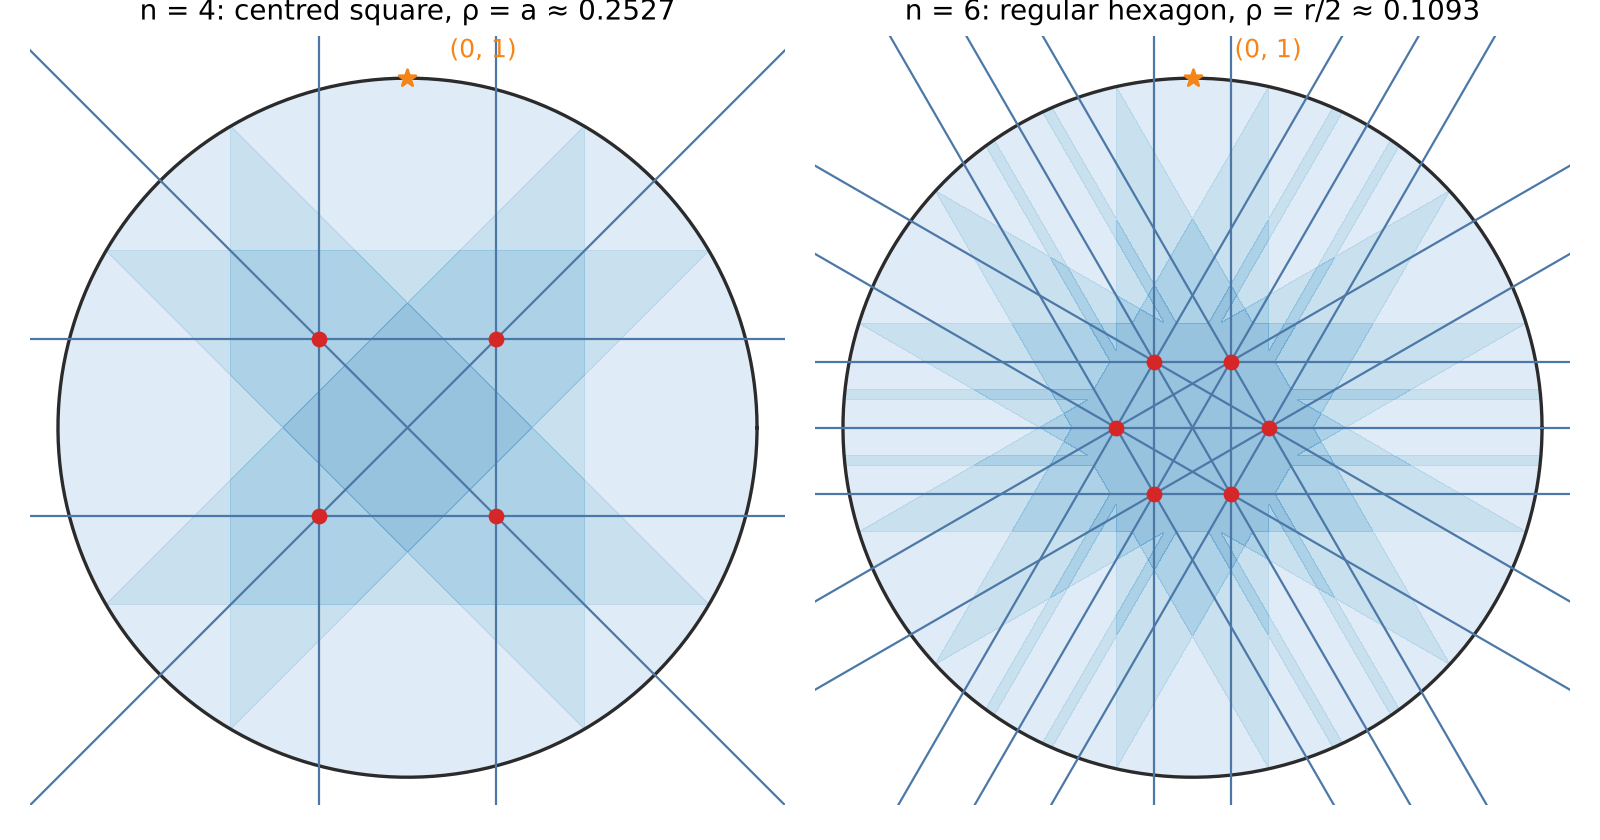
\includegraphics[width=0.8\textwidth]{figures/fig1_square_hexagon.png}
\caption{The centred square ($n=4$) and the regular hexagon ($n=6$) of Theorem~D, with their spanned
lines and the strips of half-width $\rho$ around them (darker where strips overlap). In both, $\rho$ is
attained at the boundary point $(0,1)$.}\label{fig:square}
\end{figure}

Every cluster shrinking to the centre has $\liminf\rho\ge\sin(\gamma_n/2)$: if all spanned lines pass within $r$ of
the centre, each is within $r$ of a parallel line through the centre, so $\rho\ge\sin(G/2)-r$. 

\paragraph{Extensions.} Section~\ref{sec:ext} treats four variants: great hyperspheres through $d$
points of $\Sph^d$ (Section~\ref{sec:D-spheres}), where the infimum of the angular covering radius lies
between $\pi/(2K)$ and $\pi/(2p_d(n))$; points anywhere in $\R^d$ (Section~\ref{sec:D-anywhere}), where
the infimum $\mu_d(n)$ of $\rho$ satisfies $\mu_d(d+1)=1/(d+1)$ and
$d!\le\liminf n^d\mu_d(n)\le\limsup n^d\mu_d(n)\le d^d$; the $j$-flats spanned by $j+1$ of the points
(Section~\ref{sec:D-flats}), for which the analogue $\lambda_d^{(j)}(n)$ of $\lambda_d(n)$ is
$\Theta(n^{-(j+1)/(d-j)})$; and general convex bodies (Section~\ref{sec:convex}).
Theorem~A, Corollary~1 and the small-$n$ results use the ball; Section~\ref{sec:convex} says what extends to
other convex bodies.

\section{The lower bound}\label{sec:lower}

\subsection{Bang's sign argument}\label{sec:bang}

\begin{lemma}[Bang's sign argument with a norm]\label{lem:bang}
If the closed $\eps$-slabs around hyperplanes $\{\ip{x}{u_j}=m_j\}$ with $|u_j|=1$ cover $\ball^d$, then
$\eps\cdot\max_{|v|=1}\sum_j|\ip{u_j}{v}|\ge1$.
\end{lemma}

\begin{proof}
For $\eps'>\eps$ choose signs $\sigma$ maximising $|x_\sigma|^2-2\eps'\sum\sigma_jm_j$, where
$x_\sigma=\eps'\sum\sigma_ju_j$. Flipping $\sigma_i$ changes this by
$-4\eps'[\sigma_i(\ip{x_\sigma}{u_i}-m_i)-\eps']\le0$. So $x_\sigma$ lies outside every slab, hence
outside the ball, and $1<|x_\sigma|\le\eps'\max_v\sum|\ip{u_j}{v}|$. Let $\eps'\downarrow\eps$. (This is
a one-line consequence of Bang's lemma as stated in Verreault's survey \cite{Verreault}, Lemma~2.5:
Bang's point avoids every slab, and its norm is at most $\eps'\max_v\sum|\ip{u_j}{v}|$.)
\end{proof}

In particular a covering list of $k$ hyperplanes has covering radius at least $1/k$, so
$\lambda_d(n) \ge 1/K$.

\subsection{Spanned hyperplanes never attain Bang's bound}
\label{sec:A-strict}

We prove Corollary~1, $\lambda_d(n) > 1/\binom nd$ for every $d \ge 2$ and $n > d$. The proof uses only
Lemma~\ref{lem:bang}. (For $n = d$ there is at most one hyperplane, and $\lambda_d(d) = 1 = 1/K$, attained
by $d$ independent points on a hyperplane through the centre.)

\begin{proof}[Proof of Corollary~1]
Suppose $\lambda_d(n) = 1/K$, and take labelled $n$-point sets $P_k$ with $\rho(P_k) \to 1/K$.
Pass to a subsequence along which:
\begin{enumerate}[label=(\roman*)]
  \item the family $\AI$ of affinely independent $d$-subsets (by labels) is the same for all $k$;
  \item each labelled point converges, $p_i^{(k)} \to p_i \in \ball^d$;
  \item for each $F \in \AI$, the hyperplane of $F$, written
    $\{\ip{x}{u_F^{(k)}} = m_F^{(k)}\}$ with $|u| = 1$ and $|m| \le 1$, has $u_F^{(k)} \to u_F$
    and $m_F^{(k)} \to m_F$.
\end{enumerate}
This is possible by compactness: (i) has finitely many possibilities, and $|m| \le 1$ because the
hyperplane meets $\ball^d$. The limit hyperplane $H_F = \{\ip{x}{u_F} = m_F\}$ contains $p_i$ for
every $i \in F$, by continuity of $\ip{p_i^{(k)}}{u_F^{(k)}} - m_F^{(k)} = 0$.

For $|x| \le 1$ we have $|\dist(x, H) - \dist(x, H')| \le |u - u'| + |m - m'|$. Along the
subsequence $\AH_{P_k} = \{H_F^{(k)} : F \in \AI\}$, and a min over a finite family followed by a
max over $\ball^d$ is $1$-Lipschitz in the sup norm. So the covering radius of the list
$(H_F)_{F \in \AI}$ is the limit of $\rho(P_k)$, namely $1/K$. $\AI \ne \emptyset$, since
otherwise $\rho(P_k) = \infty$. If $|\AI| < K$, Lemma~\ref{lem:bang} would give covering radius
$\ge 1/|\AI| > 1/K$ for each $P_k$ (a bound independent of $k$), contradicting
$\rho(P_k) \to 1/K$. So $|\AI| = K$: every $d$-subset is independent.

Apply Lemma~\ref{lem:bang} to the list $(H_F)$ with $\eps = 1/K$. Then
$\max_v \sum_F |\ip{u_F}{v}| \ge K$. Since each term is at most $1$ and there are $K$ terms, some
unit $v$ has $|\ip{u_F}{v}| = 1$ for all $F$. So every $H_F$ is $\{\ip{x}{v} = b_F\}$ for some
$b_F$. Their $1/K$-slabs cover $\ball^d$, in particular the diameter $\{tv : |t| \le 1\}$. So the
$K$ intervals $[b_F - 1/K,\, b_F + 1/K]$ cover $[-1, 1]$, whose length $2$ equals their total
length. Hence any two of them meet in at most one point, and the $b_F$ are pairwise distinct.

Since $n \ge d + 1$ and $d \ge 2$, the $d$-sets $F = \{1, \dots, d\}$ and
$F' = \{2, \dots, d+1\}$ are distinct and share the point $p_2$. Both $H_F$ and $H_{F'}$ contain
$p_2$, so $b_F = \ip{p_2}{v} = b_{F'}$. This is a contradiction.
\end{proof}

\begin{remark}
The limit points $p_i$ may coincide, and the limit hyperplanes need not be spanned by the limit
points. The proof uses only that $H_F$ contains $p_i$ for $i \in F$.
\end{remark}

\subsection{The tilt budget}\label{sec:tilt}

Applied to $\mathcal H_P$, Lemma~\ref{lem:bang} shows that if $\rho(P)$ is close to Bang's bound $1/K$,
then the normals are nearly parallel. To quantify this, let $\eps = \rho(P)$; if $P$ has no $d$ affinely
independent points, $\rho = \infty$ and there is nothing to prove. Here $\eps > 0$, since finitely many
hyperplanes cannot cover $\ball^d$, and the closed $\eps$-slabs $S_H$ around the $K'$ hyperplanes
$H \in \AH_P$ cover $\ball^d$, since the maximum defining
$\rho(P)$ is attained (a maximum over the compact $\ball^d$ of a minimum of finitely many continuous
functions). Apply Lemma~\ref{lem:bang} to $\AH_P$ ($k = K'$) with a maximising unit $v$. Orient each normal so that
$\cos\psi_H = \ip{u_H}{v} \ge 0$, with $\psi_H \in [0, \pi/2]$. Write
$H = \{\ip{x}{u_H} = m_H\}$; then $|m_H| \le 1$, since $H$ meets $P \subset \ball^d$. Put
$\kappa_H = 1 - \cos\psi_H \in [0, 1]$. Since $\sum_H \cos\psi_H \ge 1/\eps$,
\begin{equation}\label{eq:tilt-a}
  \sum_{H \in \AH_P} \kappa_H \le K' - 1/\eps \le K - 1/\eps,
\end{equation}
and we get the \emph{tilt budget}
\begin{equation}\label{eq:tilt}
  \sum_{Q \text{ indep}} \kappa_{H(Q)} + \#\{\text{dependent } d\text{-sets}\} \le K - \frac1\eps .
\end{equation}
Indeed,
$\sum_Q \kappa = \sum_H N_H \kappa_H \le \sum_H \kappa_H + \sum_H (N_H - 1) \le T - 1/\eps$,
where $T = \sum_H N_H$, and $\#\text{dependent} = K - T$.
The \emph{height} of $x$ is $t(x) = \ip{x}{v}$.

\subsection{Proof of Theorem~A}
\label{sec:A-unified}

\paragraph{Overview.} With $m_0$ the mean height of the points, we integrate $\Phi(x)=(t(x)-m_0)^2$
against a measure whose height is uniform on $[-1,1]$, so that $\int\Phi=1/3+m_0^2$: for $d=2$ the
Archimedes measure $dx/(2\pi\sqrt{1-|x|^2})$ (Gardner's relative-width measure of the disc
\cite{Gardner}), and for $d\ge3$ the uniform measure on $\Sph^{d-1}\cap V$ averaged over random
$3$-spaces $V\ni v$ ($V=\R^3$ when $d=3$) (Step~1). The slab of $H$ carries $\Phi$-mass at most
$\eps[G_H(m_H)+e(\psi_H)]+2\eps^2$ (Steps~2--4): steep slabs carry more mass, but they also spend more
of the tilt budget. The $d$-sets on the hyperplanes bound $\sum_HG_H(m_H)$ by $A_d(K-1/\eps)$ (Step~5),
and covering gives the bound (Step~6). Dimension $3$ is forced by the method: only on the
$2$-sphere is the height of a uniform point uniform (Archimedes); on a circle it has the arcsine law,
whose density is unbounded at $\pm1$, so a slab of half-width $\eps$ near a pole can carry mass of order
$\sqrt\eps$ rather than $\eps$.

\paragraph{Notation.} We use the notation of Sections~\ref{sec:results} and~\ref{sec:tilt}. Note
$A_2 = 5$ and $A_3 = 4$, and $\Lambda_d = A_d$ for $d \le 3$. For $d \ge 4$ put $\Abb_d = 2/(d-1)$, so that
$\Lambda_d(m) = A_d + (1+|m|)^2(C_d - 1) + 4(1+|m|)(1 - \Abb_d)$; also $C_4 = \pi/2$, $C_5 = 2$ and
$C_{d+2} = C_d (d-1)/(d-2)$.
Let $m_0$ be the mean height of $P$, so $|m_0| \le 1$.
Put $\Phi(x) = (t(x) - m_0)^2$ and $M_0 = (1 + |m_0|)^2$.

\paragraph{Step 1 (test measures with uniform height).} Each case uses a probability measure
$\sigma$ whose height $t$ is uniform on $[-1, 1]$, so $\int \Phi \, d\sigma = 1/3 + m_0^2$.
\begin{itemize}
  \item $d = 3$: $\sigma$ is uniform on $\Sph^2$. By Archimedes, for every unit $w$,
    $\ip{y}{w}$ is uniform on $[-1, 1]$, and given $\ip{y}{w} = s$ the point is uniform on the
    circle at that level.
  \item $d = 2$: $\sigma$ is the image of the uniform measure on $\Sph^2 \subset \R^3$ under the
    orthogonal projection onto $\R^2 \supset \ball^2$, which is
    $dx / (2\pi\sqrt{1 - |x|^2})$ on $\ball^2$. A slab $\{|\ip{x}{u} - m| \le \eps\}$ of $\R^2$
    pulls back to the slab of $\R^3$ with the same $u$, $m$, $\eps$, and $\Phi$ pulls back to
    the same quadratic in $\ip{y}{v}$. So every computation below for $d = 3$ applies verbatim.
  \item $d \ge 4$: let $\Pi$ be a uniformly random $2$-plane in $v^\perp$ and
    $V = \R v \oplus \Pi$. Let $\sigma_V$ be uniform on $S_V = \Sph^{d-1} \cap V$, and use
    $\sigma_V$ averaged over $\Pi$. For a unit $e \perp v$, $\beta = |P_\Pi e|^2$ has law
    $\mathrm{Beta}(1, (d-3)/2)$, being $(g_1^2 + g_2^2)/(g_1^2 + \dots + g_{d-1}^2)$ for
    independent Gaussians (here $d - 1 \ge 3$). Hence
    $\E\beta = 2/(d-1) = \Abb_d$ and
    $\E\beta^{-1/2} = \frac{d-3}{2}\, B\bigl(\frac12, \frac{d-3}{2}\bigr)
    = \sqrt\pi\,\Gamma(\frac{d-1}2)/\Gamma(\frac{d-2}2) = C_d$.
\end{itemize}
For $d \le 3$ set $V = \R^3$ and $\beta \equiv 1$ below. In every case the covering
$S_V \subset \bigcup_H S_H$, together with the uniform height on $S_V$, gives
\begin{equation}\label{eq:A-unified-2}
  \frac13 + m_0^2 \le \sum_{H \in \AH_P} \E \int_{S_H} \Phi \, d\sigma_V.
\end{equation}

\paragraph{Step 2 (one slab, one section).} Fix $H$ with $a = \cos\psi$, $b = \sin\psi$, offset
$m$, and $u = av + be$ ($e \perp v$ a unit vector, if $b > 0$). Then $P_V u = av + b P_\Pi e$, so
$r := |P_V u| = \sqrt{a^2 + \beta b^2} \in [a, 1]$, and $r > 0$ almost surely ($\beta > 0$ a.s.).
Put $\tilde u = P_V u / r$. Then
$\ip{y}{u} = r \ip{y}{\tilde u}$ on $V$, $\ip{v}{\tilde u} = a/r$ and
$1 - a^2/r^2 = \beta b^2/r^2$. By Archimedes in $V$, $\tilde s = \ip{y}{\tilde u}$ is uniform on
$[-1, 1]$, and
\begin{equation*}
  \E[\Phi \mid \tilde s] = \tilde\Gamma(\tilde s)
    = (\tilde s a/r - m_0)^2 + (1 - \tilde s^2)\, \beta b^2/(2r^2).
\end{equation*}
Since $s = r\tilde s$ has density $1/(2r)$ on $(-r, r)$, averaging over $\Pi$ (Tonelli; everything is
nonnegative) gives
\begin{equation*}
  \E \int_{S_H} \Phi \, d\sigma_V = \frac12 \int_{m-\eps}^{m+\eps} \overline G_H(s) \, ds, \qquad
  \overline G_H(s) = \E\bigl[r^{-1} \tilde\Gamma(s/r)\, \Aone\{|s| < r\}\bigr],
\end{equation*}
and $\overline G_H = 0$ for $|s| \ge 1$. For $d \le 3$, $r \equiv 1$ and
$\overline G_H(s) = G_H(s) \cdot \Aone\{|s| < 1\}$, where
\begin{equation*}
  G_H(s) = (sa - m_0)^2 + (1 - s^2)\, b^2/2.
\end{equation*}

\paragraph{Step 3 (averaging costs only tilt).} For $|s| < 1$ we have
$\overline G_H(s) \le G_H(s) + e(\psi_H)$, with $e \equiv 0$ for $d \le 3$, and for $d \ge 4$
\begin{equation*}
  e(\psi) = M_0(R(\psi) - 1) + 2(1 + |m_0|)(1 - \Abb_d)\, b^2, \qquad R(\psi) = \E[1/r].
\end{equation*}

\begin{proof}[Proof ($d \ge 4$)]
On $\{|s| < r\}$ let $\tilde c = sa/r^2$, $T = \tilde\Gamma(s/r)$ and $\omega = a/r \in [0, 1]$, so the integrand
is $r^{-1}T$.
\begin{itemize}
  \item $T \le M_0$: $|\tilde c| = (|s|/r)\omega \le \omega$ and $\beta b^2/r^2 = 1 - \omega^2$, so
    $T \le (\omega + |m_0|)^2 + (1 - \omega^2)/2$, which is non-decreasing in $\omega$ and equals $M_0$ at $\omega = 1$.
  \item $T \le G_H(s) + 2(1 + |m_0|)(1 - r^2)$: $(\tilde c - m_0)^2 - (sa - m_0)^2 = (\tilde c - sa)(\tilde c + sa - 2m_0)$
    with $|\tilde c - sa| = |\tilde c|(1 - r^2) \le 1 - r^2$ and $|\tilde c + sa - 2m_0| \le 2(1 + |m_0|)$; and
    $(1 - s^2/r^2)\beta b^2/(2r^2) \le (1 - s^2)b^2/2$, as $\beta \le r^2 \le 1$.
\end{itemize}
So $r^{-1}T = T + (r^{-1} - 1)T \le Z := G_H(s) + 2(1 + |m_0|)(1 - r^2) + M_0(r^{-1} - 1)$. $Z \ge 0$ for
$|s| \le 1$, so $\overline G_H(s) \le \E Z = G_H(s) + e(\psi)$, using $\E(1 - r^2) = b^2(1 - \Abb_d)$.
\end{proof}

\begin{lemma}[$d \ge 4$]\label{lem:R}
$R(\psi) - 1 \le (C_d - 1)\, \kappa$.
\end{lemma}

\begin{proof}
Let $a = \cos\psi < 1$ (for $a = 1$ both sides vanish) and $k = (d-3)/2$, so $\beta$ has density $k(1-x)^{k-1}$.
Substituting $x = (u^2 - a^2)/(1 - a^2)$, i.e.\ $u = r \in (a, 1)$,
\[
  R - 1 = \E\Bigl[\frac{1 - r}{r}\Bigr] = \frac{2k}{(1 - a^2)^k}N(a), \qquad N(a) = \int_a^1(1 - u)(1 - u^2)^{k-1}du,
\]
so $\varphi(a) := (R - 1)/(1 - a) = 2kN(a)/D(a)$ with $D(a) = (1 - a)(1 - a^2)^k$. At $a = 0$, with $x = u^2$,
$C_d = 2k\int_0^1(1 - u^2)^{k-1}du$ and $2k\int_0^1u(1 - u^2)^{k-1}du = 1$, so $\varphi(0) = C_d - 1$. On $[0, 1)$,
$N' = -(1 - a)(1 - a^2)^{k-1}$ and $D' = -(1 - a^2)^{k-1}(1 - a)(1 + (2k + 1)a)$, so
$N'D - ND' = -(1 - a)(1 - a^2)^{k-1}Q$ with $Q = D - (1 + (2k+1)a)N$. Then $Q' = -(2k + 1)N \le 0$ (the other terms
cancel) and $Q(a) \to 0$ as $a \to 1$, so $Q \ge 0$, $\varphi' \le 0$ and $\varphi(a) \le \varphi(0) = C_d - 1$.
\end{proof}

With $b^2 \le 2\kappa$ this gives $e(\psi_H) \le (\Lambda_d(m_0) - A_d)\, \kappa_H$ for all $d$.

\paragraph{Step 4 (one slab).} (For $d = 2$, $S_H$ here is the pull-back slab in $\R^3$.) On
$[-1, 1]$,
$|G_H'(s)| = |2a(sa - m_0) - sb^2| \le 2a(a + 1) + b^2 = (1 + a)^2 \le 4$. Since $|m| \le 1$, the
segment between $m$ and any $s \in [-1, 1]$ stays in $[-1, 1]$, so the Lipschitz bound applies; and
$G_H(m) + e \ge 0$ covers the part of the slab outside $[-1, 1]$:
\begin{equation*}
  \E \int_{S_H} \Phi \, d\sigma_V
    \le \frac12 \int_{m-\eps}^{m+\eps} \bigl(G_H(m) + e + 4|s - m|\bigr)\, ds
    = \eps\bigl[G_H(m) + e(\psi_H)\bigr] + 2\eps^2.
\end{equation*}

\paragraph{Step 5 ($d$-sets).} For a $d$-set $Q$ let $X_Q = (\text{mean height of } Q) - m_0$, and
let $V_Q$ be the population variance of its heights (mean squared deviation, dividing by $d$).
With $\delta_p = t_p - m_0$ (so $\sum_p \delta_p = 0$), counting over all $d$-sets gives
\begin{equation*}
  \sum_Q X_Q^2 = \binom{n-2}{d-1} \frac{\sum_p \delta_p^2}{d^2}, \qquad
  \sum_Q V_Q = \Bigl[\binom{n-1}{d-1}\Big/d - \binom{n-2}{d-1}\Big/d^2\Bigr] \sum_p \delta_p^2,
\end{equation*}
so
\begin{equation*}
  \sum_Q X_Q^2 = \frac{n - d}{(d - 1)n} \sum_Q V_Q.
\end{equation*}
For an independent $Q \subset H$, put $c_H = m_H \cos\psi_H$ and
$Y_Q = c_H - (\text{mean height of } Q)$. Write a point of $H$ as $z = m_H u_H + z'$ with
$z' \perp u_H$, and let $e'$ be the unit vector in the direction of $v - \cos\psi_H\, u_H$ (any unit
vector $\perp u_H$ if $\psi_H = 0$). Then $\ip{z}{v} = c_H + b\ip{z'}{e'}$, with $b = \sin\psi_H$.
The points $p$ of $Q$ lie in $H \cap \ball^d$, so $|z'_p|^2 \le 1 - m_H^2$, and their heights are
$c_H + b\,\sigma_p$ with $\sigma_p = \ip{z'_p}{e'}$, $\sigma_p^2 \le 1 - m_H^2$. So $Y_Q = -b\,\bar\sigma$
and $V_Q = b^2 \operatorname{Var}(\sigma)$ (mean and population variance over $p \in Q$), and since a
mean square is the squared mean plus the variance,
\begin{equation*}
  Y_Q^2 + V_Q = b^2 \cdot \tfrac1d \textstyle\sum_{p \in Q} \sigma_p^2 \le w_H^2 := (1 - m_H^2)\, b^2 .
\end{equation*}
Since $c_H - m_0 = X_Q + Y_Q$ and, by Cauchy--Schwarz with weights $\frac1d + \frac{d-1}d = 1$,
$(X + Y)^2 \le d X^2 + \frac{d}{d-1} Y^2$, every independent $Q \subset H$ has
\begin{equation*}
  G_H(m_H) = (X_Q + Y_Q)^2 + \tfrac12 w_H^2 \le T_Q := d X_Q^2 + \tfrac{d}{d-1}\bigl(w_H^2 - V_Q\bigr)
    + \tfrac12 w_H^2 .
\end{equation*}
Now sum, in three steps.
\begin{itemize}
  \item \emph{From hyperplanes to $d$-sets.} Pick one independent $Q_H \subset H$ for each
    $H \in \AH_P$. Every $T_Q \ge G_{H(Q)}(m_{H(Q)}) \ge 0$, so
    $\sum_H G_H(m_H) \le \sum_H T_{Q_H} \le \sum_{Q \text{ indep}} T_Q$.
  \item \emph{The cancellation.} Split
    $\sum_{Q \text{ indep}} T_Q = \bigl(\frac{d}{d-1} + \frac12\bigr) \sum_{Q \text{ indep}} w_{H(Q)}^2
    + \Delta$ with $\Delta = d \sum_{Q \text{ indep}} X_Q^2 - \frac{d}{d-1} \sum_{Q \text{ indep}} V_Q$.
    By the variance identity, $(n - d)/n \le 1$ and $V_Q \ge 0$,
    \begin{equation*}
      d \sum_{Q \text{ indep}} X_Q^2 \le d \sum_{\text{all } Q} X_Q^2
        = \frac{d}{d-1}\cdot\frac{n-d}{n} \sum_{\text{all } Q} V_Q \le \frac{d}{d-1} \sum_{\text{all } Q} V_Q ,
    \end{equation*}
    so $\Delta \le \frac{d}{d-1} \sum_{Q \text{ dep}} V_Q \le \frac{d}{d-1}\,\Adep$, since heights lie in
    $[-1, 1]$ and so $V_Q \le 1$.
  \item \emph{The tilt budget.} $w_H^2 \le b^2 = (1 - \cos\psi_H)(1 + \cos\psi_H) \le 2\kappa_H$, so
    $\bigl(\frac{d}{d-1} + \frac12\bigr) w_H^2 \le \frac{3d-1}{d-1}\kappa_H = A_d \kappa_H$; and
    $\frac{d}{d-1} \le A_d$.
\end{itemize}
Hence, by \eqref{eq:tilt},
\begin{equation*}
  \sum_H G_H(m_H) \le A_d \Bigl(\sum_{Q \text{ indep}} \kappa_{H(Q)} + \Adep\Bigr) \le A_d (K - 1/\eps).
\end{equation*}
(For $d = 2$ every pair is independent, so $\Delta \le 0$.)

\paragraph{Step 6 (conclusion).} By \eqref{eq:A-unified-2}, Steps 3--5 and \eqref{eq:tilt-a}, with
$I = 1/3 + m_0^2$ and $\Lambda = \Lambda_d(m_0)$:
\begin{equation*}
  I \le \Lambda(K\eps - 1) + 2K\eps^2
\end{equation*}
(the slab errors $2\eps^2$ number $K' \le K$). So $K\eps \ge (1 + I/\Lambda)/(1 + 2\eps/\Lambda) \ge (1 + q_d)/(1 + 2\eps/A_d)$, since
$I/\Lambda \ge q_d$ and $\Lambda \ge A_d$. For the liminf: $f(x) = x(1 + 2x/A_d)$ is increasing
and continuous, so $f(\lambda_d(n)) \ge (1 + q_d)/\binom{n}{d}$ although the infimum need not be
attained. If $L = \liminf n^d \lambda_d(n) = \infty$ there is nothing to prove. Otherwise, along a
sequence $n_k$ with $n_k^d \lambda_d(n_k) \to L < \infty$ we get $\lambda_d(n_k) \to 0$, so
\begin{equation*}
  L = \lim n_k^d \lambda_d(n_k)
    \ge \lim \frac{(1 + q_d)\, n_k^d}{\binom{n_k}{d}\bigl(1 + 2\lambda_d(n_k)/A_d\bigr)}
    = d!\,(1 + q_d). \tag*{\qedsymbol}
\end{equation*}

\paragraph{Constants.} $q_2 = (1/3)/5$ and $q_3 = (1/3)/4$ (the minimum is at $m = 0$), so
$(1 + 1/15)/(1 + 2\rho/5) = 16/(15 + 6\rho)$ and $(1 + 1/12)/(1 + \rho/2) = 13/(12 + 6\rho)$.

\subsection{\texorpdfstring{The constants for $d \ge 4$: a hand proof of $q_d \ge 0.08/\sqrt{d-2}$}%
{The constants for d >= 4: a hand proof of q\_d >= 0.08/sqrt(d-2)}}
\label{sec:A-qd}

Here $d \ge 4$. Since $\Lambda_d$ depends only on $|m|$, the minimum defining $q_d$ may be taken over
$m \in [0, 1]$, where $1 + |m| = 1 + m$.

\begin{proposition}\label{prop:A-qd}
For every $d \ge 4$, $q_d \ge 0.08/\sqrt{d-2}$. Moreover $q_4 \ge 0.0588$ and $q_5 \ge 0.0496$.
\end{proposition}

\begin{proof}
\emph{Preliminaries.} $\Lambda_d(m) \ge A_d > 0$, since $C_d \ge 1$ and $\Abb_d \le 1$. So for $q, s > 0$,
\begin{equation}\label{eq:A-qd-crit}
  s(1/3 + m^2) - q\Lambda_d(m) \ge 0 \text{ for all } m \in [0, 1]
  \quad\Longrightarrow\quad q_d \ge q/s.
\end{equation}
$\Lambda_d$ increases with $C_d$ (its coefficient $(1+m)^2$ is positive), so in
\eqref{eq:A-qd-crit} $C_d$ may be replaced by an upper bound. With
$\Lambda_d(m) = a_2 m^2 + a_1 m + a_0$, where $a_2 = C_d - 1$, $a_1 = 2(C_d - 1) + 4(1 - \Abb_d)$ and
$a_0 = A_d + (C_d - 1) + 4(1 - \Abb_d)$, the left side of \eqref{eq:A-qd-crit} is the quadratic
$Q(m) = Q_2m^2 + Q_1m + Q_0$ with $Q_2 = s - qa_2$, $Q_1 = -qa_1$, $Q_0 = s/3 - qa_0$; it is $\ge 0$ on
$\R$ when $Q_2 > 0$ and $Q_1^2 - 4Q_2Q_0 < 0$. We use $\pi < 3.1416$ and $A_d = 3 + 2/(d-1)$.

\emph{Small $d$.} From $\Gamma(\frac32) = \sqrt\pi/2$ and $\Gamma(\frac52) = 3\sqrt\pi/4$:
$C_4 = \pi/2$, $C_5 = 2$, $C_6 = 3\pi/4$, $C_7 = 8/3$. With $C_d$ replaced by the stated bound:
\begin{center}
\small
\begin{tabular}{cccccccc}
\toprule
$d$ & bound for $C_d$ & $q$ & $s$ & $Q_2$ & $Q_1$ & $Q_0$ & $Q_1^2 - 4Q_2Q_0$\\
\midrule
4 & $1.5708$ & $0.0588$ & $1$ & $0.966437$ & $-0.145526$ & $0.005770$ & $-0.00113$\\
5 & $2$ & $0.0496$ & $1$ & $0.950400$ & $-0.198400$ & $0.010933$ & $-0.00220$\\
6 & $2.3562$ & $0.08$ & $2$ & $1.891504$ & $-0.408992$ & $0.094171$ & $-0.545$\\
7 & $8/3$ & $0.08$ & $2.236$ & $2.102667$ & $-0.480000$ & $0.132000$ & $-0.880$\\
\bottomrule
\end{tabular}
\end{center}
(Entries are exact rationals rounded to six places.) Since $2.236 \le \sqrt5$, this gives $q_4 \ge 0.0588 \ge 0.08/\sqrt2$, $q_5 \ge 0.0496 \ge 0.08/\sqrt3$ (as
$2 \cdot 0.0588^2$ and $3 \cdot 0.0496^2$ exceed $0.0064$), $q_6 \ge 0.08/2$ and $q_7 \ge 0.08/\sqrt5$.

\emph{All $d \ge 8$ at once.} Put $x = \sqrt{d-2} \ge \sqrt6$.
\begin{enumerate}[label=(\alph*)]
  \item $C_d - 1 \le C_d \le \sqrt{\pi/2}\, x$: with $y = (d-2)/2$, log-convexity of $\Gamma$
    (H\"older) gives $\Gamma(y + \frac12) \le \Gamma(y)^{1/2}\Gamma(y+1)^{1/2} = \sqrt y\,\Gamma(y)$,
    so $C_d \le \sqrt{\pi y}$.
  \item $A_d/x = (3d-1)/((d-1)\sqrt{d-2}) \le 23/(7\sqrt6)$, as $3 + 2/(d-1)$ and $1/\sqrt{d-2}$
    decrease.
  \item $(1 - \Abb_d)/x = (d-3)/((d-1)\sqrt{d-2}) \le 5/(7\sqrt6)$: squared, this is
    $294(d-3)^2 \le 25(d-1)^2(d-2)$, and with $e = d - 8 \ge 0$ the difference is
    $25e^3 + 206e^2 + 385e \ge 0$.
  \item $1/\sqrt6 \le 0.40825$ and $\sqrt{\pi/2} \le 1.2534$ ($0.40825^2 \ge 1/6$,
    $1.2534^2 > 1.5708$).
\end{enumerate}
So $\Lambda_d(m)/x \le \frac{23}{7}(0.40825) + 1.2534(1+m)^2 + \frac{20}{7}(0.40825)(1+m)$,
and \eqref{eq:A-qd-crit} with $s = x$, $q = 0.08$ follows from $Q(m) \ge 0$ for the quadratic with
$Q_2 = 1 - 0.08 \cdot 1.2534 = 0.899728$, $Q_1 = -0.08(2 \cdot 1.2534 + \frac{20}{7} \cdot 0.40825)
= -0.293858\ldots$ and $Q_0 = \frac13 - 0.08(\frac{23}{7} \cdot 0.40825 + 1.2534 +
\frac{20}{7} \cdot 0.40825) = 0.032436\ldots$, whose discriminant is
$0.086352\ldots - 0.116733\ldots < 0$.
\end{proof}

The arithmetic is re-checked in exact rationals in the accompanying repository
(\nolinkurl{experiments/qd_sharp/check_qd_new.py}). Numerically, $q_d\sqrt{d-2}$ is smallest at
$d = 4$ ($\approx 0.0832$) and increases for larger $d$ towards about $0.20$.

% ======================================================================
\subsection{Sharper constants in the plane and in space}
\label{sec:A-sharp}

The proof of Theorem~A relaxes the position of the points of a $d$-set to $Y_Q^2 + V_Q \le w_H^2$
(Step~5). For $d = 2$ and $d = 3$ (where $e \equiv 0$) the exact constraint gives larger limit
constants. (The finite-$n$ inequalities below are stronger than those of Theorem~A only for small $\rho$:
for $\rho < 113/1650$ when $d = 2$ and $\rho < 7/120$ when $d = 3$.)

\begin{proposition}\label{prop:A-sharp}
Let $n \ge d$, and let $\rho = \rho(P)$ ($= \infty$ if $P$ has no $d$ affinely independent points, when there is
nothing to prove). Every $n$-point $P \subset \ball^2$ satisfies $\binom n2\rho\,\bigl(\frac{3161}{3432} + \frac{8\rho}{13}\bigr) \ge 1$,
and every $n$-point $P \subset \ball^3$ satisfies $\binom n3\rho \ge 70/(63 + 60\rho)$. Hence
\[
  \liminf_n n^2\lambda_2(n) \ge \frac{6864}{3161} = 2.17146\ldots,
  \qquad
  \liminf_n n^3\lambda_3(n) \ge \frac{20}{3}.
\]
\end{proposition}

We use the notation of Section~\ref{sec:A-unified} with $d \in \{2, 3\}$, and write
$G_H = G_H(m_H) = (c_H - m_0)^2 + w_H^2/2$.

\paragraph{The framework.} By Step~5, every point of $H \cap \ball^d$ has height in
$[h_1, h_2]$ with $h_{1,2} = c_H \mp w_H$. Fix $A, B > 0$, $C = \gamma m_0$ and $C_0, \lambda_0 \ge 0$,
and suppose that for every independent $d$-set $Q$ on a hyperplane $H \in \AH_P$
\begin{equation}\label{eq:A-sharp-star}
  G_H - B\bigl((d-1)X_Q^2 - V_Q\bigr) - C X_Q - A\kappa_H \le C_0 + \lambda_0 m_0^2,
\end{equation}
and that $\tau_Q := -B((d-1)X_Q^2 - V_Q) - CX_Q \le A$ for every dependent $d$-set (for $d = 2$ there is
none). Summing \eqref{eq:A-sharp-star} over the independent $d$-sets (each $H$ carries one, and
$G \ge 0$), and using $\sum_{\text{all }Q}((d-1)X_Q^2 - V_Q) \le 0$ and $\sum_{\text{all }Q}X_Q = 0$
(Step~5) and \eqref{eq:tilt},
\[
  \sum_{H \in \AH_P} G_H \le A\Bigl(\sum_{Q\text{ indep}}\kappa_{H(Q)} + \Adep\Bigr) + K(C_0 + \lambda_0m_0^2)
    \le A(K - 1/\eps) + K(C_0 + \lambda_0m_0^2).
\]
With \eqref{eq:A-unified-2} and Steps~2 and~4 ($e \equiv 0$), $I \le \sum_H(\eps G_H + 2\eps^2)$, where
$I = 1/3 + m_0^2$. Put $\alpha = 1 - 1/(K\eps)$; dividing by $K\eps$ gives
$I(1 - \alpha) \le A\alpha + C_0 + \lambda_0m_0^2 + 2\eps$, i.e.
\begin{equation}\label{eq:A-sharp-alpha}
  \alpha \ge \frac{1/3 - C_0 + (1 - \lambda_0)m_0^2 - 2\eps}{A + 1/3 + m_0^2}.
\end{equation}

\paragraph{Reduction of \eqref{eq:A-sharp-star}.} Let $x_1, \dots, x_d$ be the heights of the points of
$Q$ minus $m_0$, and $e_2 = \sum_{i<j}x_ix_j$. Then $(d-1)X^2 - V = \frac2d e_2$, so the left side of
\eqref{eq:A-sharp-star} is $f - A\kappa_H$ with $f = G_H - \frac{2B}{d}e_2 - \frac{\gamma m_0}{d}\sum_i x_i$.
Since $f$ is affine in each $x_i \in [h_1 - m_0, h_2 - m_0]$, its maximum is at $j$ points at $h_1$ and
$d - j$ at $h_2$, $0 \le j \le d$. Expanding in $m_0$, $f = f_0 + m_0L + k_2m_0^2$ with $f_0$, $L$
not depending on $m_0$; for $\mu > 0$, $m_0L \le \mu m_0^2 + L^2/(4\mu)$, so
$f \le \Psi + (\mu + k_2)m_0^2$ with $\Psi = f_0 + L^2/(4\mu)$; we take $\lambda_0 \ge \mu + k_2$ (in both cases
below $\mu + k_2 = \frac79 \ge 0$). In terms of $D = c_H = (h_1 + h_2)/2$
and $w = (h_2 - h_1)/2$, $\Psi$ is a quadratic form $pD^2 + 2\zeta Dw + qw^2$, and $j \mapsto d - j$ changes the
sign of $\zeta$. Writing $m_H = \cos\phi$, $(D, w) = (c\cos\phi, s\sin\phi)$ with $c = \cos\psi_H$,
$s = \sin\psi_H$, so $\Psi = \mathbf w^T M\mathbf w$ with $\mathbf w = (\cos\phi, \sin\phi)$ and
$M = \bigl[\begin{smallmatrix} pc^2 & \zeta cs\\ \zeta cs & qs^2\end{smallmatrix}\bigr]$. Hence
\eqref{eq:A-sharp-star} holds if $N = (C_0 + A\kappa)\,\mathrm{Id} - M \succeq 0$, i.e. if
$N_{11}, N_{22}, \det N \ge 0$, where $\kappa = 1 - c$ and $s^2 = 2\kappa - \kappa^2$.

\paragraph{The plane.} Take $A = \frac{35}{12}$, $B = \frac43$, $\gamma = -\frac23$, $\mu = \frac{16}{9}$,
so $k_2 = -1$, $\lambda_0 = \frac79$, $C_0 = \frac{27}{352}$.
\begin{itemize}
  \item $j = 1$ (one point at each end): $L = \frac23(h_1 + h_2)$ and
    $\Psi = -\frac{1}{48}(h_1 + h_2)^2 + \frac{11}{24}(h_2 - h_1)^2 \le \frac{11}{6}w^2 \le \frac{11}{6}(1 - c^2)$,
    and $\frac{11}{6}(1 - c^2) - A\kappa = C_0 - \frac{11}{6}(\kappa - \frac{9}{44})^2 \le C_0$.
  \item $j = 2$ (both at $h_1$): $L = \frac73h_1 - h_2$ and
    $\Psi = -\frac{1}{12}D^2 + \frac{17}{12}Dw + \frac{35}{48}w^2$. Then
    $N_{11} = C_0 + A\kappa + c^2/12 > 0$, $N_{22} = \frac{27}{352} + \frac{35}{24}\kappa + \frac{35}{48}\kappa^2 > 0$,
    and $1056^2\det N = 627264\kappa^4 + 133584\kappa^3 + 7406938\kappa^2 - 623524\kappa + 13689 > 0$ for
    $\kappa \ge 0$, since $623524^2 - 4 \cdot 7406938 \cdot 13689 = -16792118552 < 0$.
  \item $j = 0$: as $j = 2$ with $\zeta \mapsto -\zeta$.
\end{itemize}
By \eqref{eq:A-sharp-alpha}, $\alpha \ge (\frac{271}{1056} + \frac29m_0^2 - 2\eps)/(\frac{13}{4} + m_0^2)
\ge \frac{271}{3432} - \frac{8\eps}{13}$, because $x \mapsto (\frac{271}{1056} + \frac29x)/(\frac{13}{4} + x)$
is increasing ($\frac29 \cdot \frac{13}{4} > \frac{271}{1056}$). This is
$\binom n2\eps(\frac{3161}{3432} + \frac{8\eps}{13}) \ge 1$.

\paragraph{Space.} Take $A = 2$, $B = \frac89$, $\gamma = -\frac{13}{9}$, $\mu = 3$, so
$k_2 = -\frac{20}{9}$, $\mu + k_2 = \frac79$; we take $\lambda_0 = \frac{9}{10} \ge \frac79$, which makes the
bound on $\alpha$ below independent of $m_0$,
$C_0 = \frac1{10}$.
\begin{itemize}
  \item $j = 3$: $L = 4h_1 - h_2$ and $\Psi = -\frac{1}{36}D^2 + \frac{19}{18}Dw + \frac{29}{36}w^2$.
    $N_{11} = \frac{23}{180} + \frac{35}{18}\kappa + \frac{\kappa^2}{36}$,
    $N_{22} = \frac1{10} + \frac7{18}\kappa + \frac{29}{36}\kappa^2$, and
    $5400\det N = 1625\kappa^4 + 2500\kappa^3 + 12175\kappa^2 - 1690\kappa + 69 > 0$ for $\kappa \ge 0$,
    since $1690^2 - 4 \cdot 69 \cdot 12175 < 0$.
  \item $j = 2$: $L = \frac73h_1 + \frac23h_2$ and $\Psi = -\frac{1}{36}D^2 + \frac{19}{54}Dw + \frac{143}{108}w^2$.
    $N_{11}$ is as before, $N_{22} = \frac1{10} - \frac{35}{54}\kappa + \frac{143}{108}\kappa^2 > 0$
    (negative discriminant), and
    \[
      145800\det N = 9875\kappa^4 + 354700\,\kappa\bigl(\kappa - \tfrac{11}{50}\bigr)^2 + 19953\kappa^2
        - \tfrac{247937}{25}\kappa + 1863 > 0,
    \]
    the last quadratic having discriminant $-31458341531/625 < 0$.
  \item $j = 0, 1$: as $j = 3, 2$ with $\zeta \mapsto -\zeta$.
  \item Dependent triples: their heights lie in $[-1, 1]$ and $\tau_Q$ is affine in each, so at the
    maximum the heights are $v \in \{\pm1\}^3$, where
    $\tau = -\frac{16}{27}e_2(v) + \frac53m_0s_1(v) - \frac{29}{9}m_0^2$ with $s_1(v) = v_1 + v_2 + v_3$. If
    $e_2(v) = -1$, $|s_1(v)| = 1$ and $\tau \le \frac{16}{27} + \frac{25}{116}$; if $e_2(v) = 3$, $|s_1(v)| = 3$
    and $\tau \le -\frac{16}{9} + \frac{225}{116}$. Both are $< 2 = A$.
\end{itemize}
By \eqref{eq:A-sharp-alpha}, $\alpha \ge (\frac{7}{30} + \frac{m_0^2}{10} - 2\eps)/(\frac73 + m_0^2)
= \frac1{10} - 2\eps/(\frac73 + m_0^2) \ge \frac1{10} - \frac{6\eps}{7}$, i.e.
$\binom n3\eps(\frac9{10} + \frac{6\eps}7) \ge 1$, which is $\binom n3\rho \ge 70/(63 + 60\rho)$.

\paragraph{The liminf.} In both cases $g(x) = x(1 - \beta_0 + \eta x)$ ($\beta_0 = \frac{271}{3432}$,
$\eta = \frac8{13}$, resp.\ $\beta_0 = \frac1{10}$, $\eta = \frac67$) is increasing, so
$g(\lambda_d(n)) \ge 1/\binom nd$, and as in Step~6 $\liminf n^d\lambda_d(n) \ge d!/(1 - \beta_0)$, which is
$6864/3161$ and $20/3$. \qed

\begin{remark}
The parameters were found by a floating-point search; the proof does not depend on it, and the
identities above are re-checked symbolically in the accompanying repository
(\nolinkurl{experiments/planar_hand/}, \nolinkurl{experiments/theoremA_d3_hand/}). The search suggests that
this method gives at most about $2.1722$ in the plane and $6.687$ in space, and only small gains for
$d \ge 4$, where the averaging error $e(\psi)$ of Step~3 dominates.
\end{remark}

\section{Constructions}\label{sec:upper}

\subsection{Flat clusters}\label{sec:B-lemma2}

The following lemma holds for $j$-flats with any base points $t_i$ that affinely span $\R^{j-1}$;
Lemma~\ref{D:M2} in Section~\ref{sec:D-flats} is the special case of moment-curve $t$'s.

\paragraph{Definitions.}
\begin{itemize}
  \item $1 \le j \le d-1$ and $m = d-j+1$. Write $\R^d = \R^{j-1} \times \R^m$, where $\R^0$ is a
    point.
  \item For a finite nonempty set $W \subset \R^m \setminus \{0\}$,
    $\delta(W) = \max_{y \in \Sph^{m-1}} \min_{w \in W} \angle(y, \pm w) \in [0, \pi/2]$, where
    $\angle(y, \pm w)$ is the smaller of the angles to $w$ and $-w$, i.e.\ the angle to the line
    $\R w$. It depends only on the lines $\R w$, so the scaling of each $w_F$ (fixed only up to
    scale, like $c$) does not matter.
  \item For a family $\mathcal{L}$ of affine subspaces,
    $\rho(\mathcal{L}) = \max_{x \in \ball^d} \min_{L \in \mathcal{L}} \dist(x, L)$.
\end{itemize}

\begin{lemma}[Flat clusters]\label{lem:B-lemma2-flats}
Let $t_0, \dots, t_j \in \R^{j-1}$ affinely span $\R^{j-1}$. Then the affine dependencies of the
$t_i$ form a line, spanned by some $c = (c_0, \dots, c_j) \ne 0$ with $\sum c_i = 0$ and
$\sum c_i t_i = 0$. Let $a_0, \dots, a_j \in \R^m$ with $w = \sum c_i a_i \ne 0$, and for $s > 0$
put $q_i = (t_i, s a_i)$. Then:
\begin{enumerate}[label=(\roman*)]
  \item the $q_i$ are affinely independent for every $s > 0$;
  \item as $s \to 0$, their $j$-flat $\Phi_s$ converges to the linear subspace
    $L_w = (\R^{j-1} \times \{0\}) \oplus \R(0, w)$, in the sense that
    $\dist(\cdot, \Phi_s) \to \dist(\cdot, L_w)$ uniformly on $\ball^d$;
  \item for any finite nonempty family of such $(j+1)$-sets, all with the same $s$, with
    directions $W = \{w_F\}$, the limit as $s \to 0$ of $\rho$ of their flats is
    $\rho(\{L_w : w \in W\}) = \sin \delta(W)$. For $j = d-1$ ($m = 2$) this is $\sin(G/2)$, with
    $G$ the largest gap mod $\pi$ of the directions of the $w_F$ (the wrap-around gap included; a
    single direction gives $G = \pi$).
\end{enumerate}
\end{lemma}

\begin{proof}
\emph{The dependency.} Since the $t_i$ affinely span $\R^{j-1}$, the $(j+1) \times j$ matrix with
rows $(1, t_i)$ has rank $j$. So its left kernel, the space of dependencies, is one-dimensional.

\emph{(i)} An affine dependency $\mu$ of the $q_i$ ($\sum \mu_i = 0$, $\sum \mu_i q_i = 0$) is in
particular a dependency of the $t_i$, so $\mu = \lambda c$. Its $\R^m$-part is then
$s \lambda w = 0$, so $\lambda = 0$.

\emph{Direction space.} The direction space $D_s$ of $\Phi_s$ contains
$\sum_i c_i q_i = (0, s w)$, a combination of the differences $q_i - q_{i_0}$ because
$\sum c_i = 0$. Hence $D_s$ contains $(0, w)$. Since $c \ne 0$ and $\sum c_i = 0$, $c$ has at least
two nonzero entries; pick $i_1$ with $c_{i_1} \ne 0$ and any $i_0 \ne i_1$.
\begin{itemize}
  \item The vectors $t_i - t_{i_0}$ ($i \ne i_0$) span $\R^{j-1}$, so the space of linear relations
    among these $j$ vectors is one-dimensional. It contains $(c_i)_{i \ne i_0}$, because
    $\sum_{i \ne i_0} c_i (t_i - t_{i_0}) = \sum_i c_i t_i - (\sum_i c_i) t_{i_0} = 0$, and that
    vector is nonzero since $c_{i_1} \ne 0$. A relation among the remaining $j-1$ vectors would be a
    relation with zero $i_1$-coefficient, hence $0$. So dropping $i = i_1$ leaves a basis of
    $\R^{j-1}$.
  \item Hence the $j$ vectors $v_i(s) = q_i - q_{i_0}$ ($i \notin \{i_0, i_1\}$) and $(0, w)$ are
    independent, so they are a basis of $D_s$ (which has dimension $j$ by (i)).
  \item As $s \to 0$ they converge to $(t_i - t_{i_0}, 0)$ and $(0, w)$, a basis of the direction
    space of $L_w$.
\end{itemize}

\emph{(ii)} The orthogonal projector $\Pi_s = B_s (B_s^{\mathsf T} B_s)^{-1} B_s^{\mathsf T}$ onto
$D_s$ ($B_s$ the matrix of the basis) depends continuously on the basis, so it converges to the
projector $\Pi$ onto $\R^{j-1} \times \{0\} \oplus \R(0, w)$. The base point
$q_{i_0} \to (t_{i_0}, 0) \in L_w$. For $\abs{x} \le 1$,
$\dist(x, \Phi_s) = \abs{(I - \Pi_s)(x - q_{i_0})}$, and its difference from the limit is at most
$\norm{\Pi_s - \Pi} \cdot (1 + \abs{q_{i_0}}) + \abs{q_{i_0} - (t_{i_0}, 0)}$ (using
$\abs{x - q_{i_0}} \le 1 + \abs{q_{i_0}}$, $\norm{I - \Pi} \le 1$ for the orthogonal projector $\Pi$,
and $\abs{q_{i_0}} \le \abs{t_{i_0}} + s\abs{a_{i_0}}$ bounded as $s \to 0$), so it
converges uniformly to
$\abs{(I - \Pi)(x - (t_{i_0}, 0))} = \dist(x, L_w)$, since $L_w$ is linear and contains
$(t_{i_0}, 0)$.

\emph{(iii)} $\rho$ of a finite family is a max over $x$ of a min of finitely many functions; if
each function moves by at most $\eta$ uniformly, the max-min moves by at most $\eta$. So it
converges when they converge uniformly. For linear $L_w$ and
$x = (x_1, x_2) \in \R^{j-1} \times \R^m$, $\dist(x, L_w) = \abs{x_2} \sin \angle(x_2, \R w)$
($0$ if $x_2 = 0$). The max over $\abs{x} \le 1$ of $\min_w$ is attained with $x_1 = 0$ and
$\abs{x_2} = 1$, and equals $\max_y \min_w \sin \angle(y, \pm w) = \sin \delta(W)$, since $\sin$ is
increasing on $[0, \pi/2]$. For $m = 2$, $\delta(W)$ is half the largest gap between the
directions mod $\pi$, so the limit is $\sin(G/2)$.
\end{proof}

\subsection{Proof of Theorem~B}\label{sec:thmB}

\begin{proof}[Proof of Theorem B]
Let $S=\{s_j\}\subset\Z_N$ be as in the theorem. Put $\theta_j=\pi s_j/N+\delta$ with
$0<\delta<\pi/N$, and $\tau_j=-\cot\theta_j$. Identify $\mathbb C$ with $\R^2$, and for $r>0$ put
$q_j=\bigl(\kappa\cdot(\tau_j,\dots,\tau_j^{d-2}),\,r/(i-\tau_j)\bigr)\in\R^{d-2}\times\R^2$, where
$\kappa>0$ is so small that the first $d-2$ coordinates of every $q_j$ lie in the open unit ball. We let
$r\to0$. By
Lemma~\ref{lem:B-lemma2-flats} (with $w_F\ne0$, shown below), every $d$ of the $q_j$ are affinely independent for every $r>0$.
\begin{itemize}
\item For a $d$-subset $F$, the affine dependence of the moment-curve points
$(\tau_j,\dots,\tau_j^{d-2})$, $j\in F$, is unique up to scale and has coefficients
$c_j=1/\prod_{k\in F,\,k\ne j}(\tau_j-\tau_k)$.
\item Partial fractions give
$w_F=\sum c_j/(i-\tau_j)=1/\prod(i-\tau_j)=\bigl(\prod\sin\theta_j\bigr)e^{-i\sum\theta_j}$.
\item Consequently $w_F\ne0$, and its direction is $-\sum_{j\in F}\theta_j=-d\delta-(\pi/N)\sum_{j\in F}s_j\bmod\pi$. As
$F$ varies, $\sum s_j$ runs over all of $\Z_N$, so the directions are $N$ equally spaced ones,
$G=\pi/N$, and Lemma~\ref{lem:B-lemma2-flats} gives $\rho\to\sin(\pi/2N)$.
\end{itemize}
For $d=2$ the curve $1/(i-\tau)$ is a circle, and this is the fact that a chord of a circle has
direction $(t+u)/2+\pi/2$ (Figure~\ref{fig:sums}).
The remaining assertions of Theorem~B, $n\le p_d(n)\le\binom nd$ and the existence of
$\sigma_d=\sup_{n>d}p_d(n)/n^d\le1/d!$, are Proposition~\ref{prop:B-blowup} below.
\end{proof}

\begin{figure}[t]
\centering
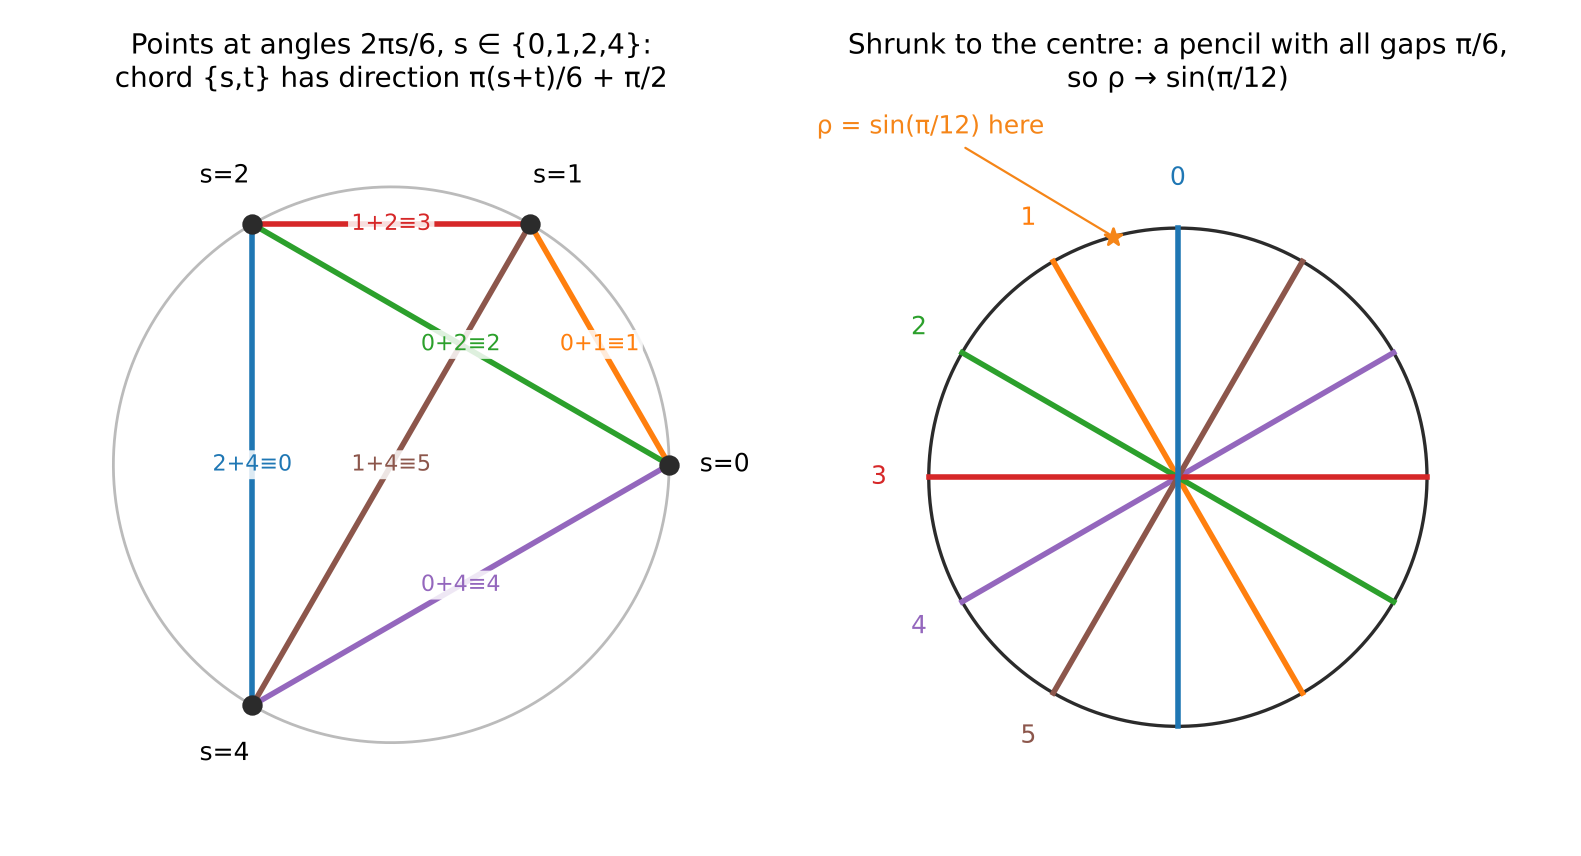
\includegraphics[width=0.85\textwidth]{figures/fig2_sums.png}
\caption{Points at angles $2\pi s/6$, $s\in\{0,1,2,4\}$, on a circle (left). The chord through $s$ and
$t$ has direction $\pi(s+t)/6+\pi/2$ (mod $\pi$: lines are unoriented), and the six pair sums hit every residue mod $6$. Shrunk to the
centre (right), the six lines form a pencil with all gaps $\pi/6$, so $\rho\to\sin(\pi/12)$. This is
the case $d=2$, $N=6$ of Theorem~B.}\label{fig:sums}
\end{figure}

% ---------------------------------------------------------------------------
\subsection{\texorpdfstring{Blow-up: $\sigma_d = \lim p_d(n)/n^d$ exists and equals $\sup$}{Blow-up: sigma\_d = lim p\_d(n)/n\^{}d exists and equals sup}}\label{sec:B-blowup}

This proves the bounds on $p_d(n)$ and the existence of $\sigma_d$ in Theorem~B.

\begin{proposition}\label{prop:B-blowup}
\leavevmode
\begin{enumerate}[label=(\alph*)]
  \item For $n \ge d+1$, $n \le p_d(n) \le \binom{n}{d}$.
  \item \emph{Seed lemma.} Let $L_0 = \{l_1, \dots, l_\ell\} \subset \Z_P$ be $\ell$ distinct
    residues such that every residue of $\Z_P$ is a sum of $d$ distinct elements of $L_0$. Then
    $\liminf_n p_d(n)/n^d \ge P/\ell^d$.
  \item Hence $\sigma_d$ exists and $\sigma_d = \sup_{n \ge d+1} p_d(n)/n^d \le 1/d!$.
\end{enumerate}
\end{proposition}

\begin{proof}
\textbf{(a) Bounds on $p_d(n)$.} For the upper bound: if $S \subset \Z_N$ with $\abs{S} = n$
works, each of the $N$ residues is the sum of some $d$-subset, so $N \le \binom{n}{d}$.

For the lower bound, take $S = \Z_n = \{0, \dots, n-1\}$. The sums of $d$ distinct elements are
all the integers from $d(d-1)/2$ to $d(d-1)/2 + d(n-d)$, which is $d(n-d) + 1$ consecutive
integers. (Starting from $\{0, \dots, d-1\}$, raise the largest element that can be raised by one,
one step at a time.) Since $d(n-d) + 1 - n = (d-1)(n-d-1) \ge 0$, they cover every residue mod
$n$. So $p_d(n) \ge n$.

\medskip
\textbf{(b) Seed lemma.}

\emph{Levels and directions.} For each $r \in \Z_P$ fix a $d$-set $J_r \subset \{1, \dots, \ell\}$
with $\sum_{j \in J_r} l_j = r$, and let $\mathcal{J} = \{J_r\}$. Fix distinct integers
$t_1, \dots, t_\ell$ and put $u_j = (1, t_j, \dots, t_j^{d-1}) \in \Z^d$. For
$J = \{j_1 < \dots < j_d\}$, let $R_J$ be the $d \times d$ matrix with columns
$u_{j_1}, \dots, u_{j_d}$. It is a Vandermonde matrix with distinct nodes, so
$D_J = \abs{\det R_J} \ge 1$. Let $Q = \lcm(P, (d-1)!, D_J : J \in \mathcal{J})$.

\emph{Moduli.} For $m \ge 1$ with $m \equiv 1 \pmod{Q}$, put $a_k = m + (k-1)Q$ for
$k = 1, \dots, d$, and $M = a_1 \cdots a_d$.
\begin{itemize}
  \item Each $a_k \equiv 1 \pmod{Q}$, so $\gcd(a_k, Q) = 1$, and hence
    $\gcd(a_k, P) = \gcd(a_k, D_J) = 1$.
  \item If a prime $p$ divides $a_i$ and $a_j$ with $i < j$, then $p \mid (j-i)Q$. Since
    $p \nmid Q$, $p \mid (j-i) \le d-1$, so $p \mid (d-1)! \mid Q$, a contradiction.
\end{itemize}
So the $a_k$ are pairwise coprime and $\gcd(M, P) = 1$.

\emph{Generators.} By the Chinese remainder theorem, $\Z_M \cong \prod_k \Z_{a_k}$. Let
$g_j \in \Z_M$ be the element with $g_j \equiv (u_j)_k \pmod{a_k}$ for every $k$. For
$J \in \mathcal{J}$ define $\varphi_J : \Z^d \to \Z_M$ by $\varphi_J(z) = \sum_s z_s g_{j_s}$.
Under the isomorphism, $\varphi_J(z)$ has $k$-th component $(R_J z)_k \bmod a_k$.

\emph{$\varphi_J$ is onto.} $\det R_J$ is coprime to $M$, so $R_J$ is invertible over $\Z_M$.
Given a target, lift its components to an integer vector $y$ with $y_k$ in the right class mod
$a_k$, and let $z \in \Z^d$ represent $R_J^{-1} y \bmod M$. Then $R_J z \equiv y \pmod{M}$ in every
coordinate. So $\ker \varphi_J$ has index $M$.

\emph{The kernel is a lattice $G_J \Z^d$.} Let $E = \operatorname{diag}(0, 1, \dots, d-1)$, so
$\operatorname{diag}(a) = mI + QE$. Put
$G_J = R_J^{-1} \operatorname{diag}(a) R_J = mI + Q \cdot R_J^{-1} E R_J$.
\begin{itemize}
  \item $R_J^{-1} = \adj(R_J)/\det R_J$ and $D_J \mid Q$, so $G_J$ has integer entries.
  \item $R_J G_J z = \operatorname{diag}(a) R_J z$, whose $k$-th coordinate is $\equiv 0 \bmod a_k$.
    So $G_J \Z^d \subset \ker \varphi_J$.
  \item $\abs{\det G_J} = \prod a_k = M$, the index of $\ker \varphi_J$. So
    $\ker \varphi_J = G_J \Z^d$.
\end{itemize}

\emph{A box meets every coset.} Every coset of $G_J \Z^d$ contains an integer point $z = G_J w$
with $w \in [0,1)^d$ (reduce $w$ mod $1$). Its $k$-th coordinate $\sum_s (G_J)_{ks} w_s$ lies in
\[
  \Bigl[\sum_{s : (G_J)_{ks} < 0} (G_J)_{ks},\ \sum_{s : (G_J)_{ks} > 0} (G_J)_{ks}\Bigr],
\]
an interval with integer endpoints and integer length $T_{J,k} = \sum_s \abs{(G_J)_{ks}}$. Row $k$
of $G_J$ is nonzero ($\det G_J = \pm M \ne 0$), and $w_s < 1$, so at least one endpoint is not
attained: the left one if row $k$ has a negative entry, the right one if it has a positive entry.
So at most $T_{J,k}$ integers occur, and they are consecutive. Put
$T = \max_{J \in \mathcal{J}, k} T_{J,k}$.
\begin{itemize}
  \item Write $[0, T)^d$ for the integer points $\{0, \dots, T-1\}^d$, and let $b_J \in \Z^d$ have
    $k$-th coordinate the least integer that occurs above. Then $b_J + [0, T)^d$ meets every coset,
    so $\varphi_J(b_J + [0,T)^d) = \Z_M$, and hence $\varphi_J([0,T)^d) = \Z_M$.
  \item With $X_j = \{i \cdot g_j : 0 \le i < T\} \subset \Z_M$, this says
    $X_{j_1} + \dots + X_{j_d} = \Z_M$ for every $J \in \mathcal{J}$.
  \item Moreover $T \le m + C$, where
    $C = Q \cdot \max_{J,k} \sum_s \abs{(R_J^{-1} E R_J)_{ks}}$ does not depend on $m$.
\end{itemize}

\emph{Lift.} $\gcd(P, M) = 1$, so $\Z_P \times \Z_M \cong \Z_{PM}$. Let
$S = \{(l_j, x) : 1 \le j \le \ell,\ x \in X_j\}$, so $\abs{S} \le \ell T$. Take
$(r, h) \in \Z_P \times \Z_M$ and $J = J_r = \{j_1 < \dots < j_d\}$. Write
$h = x_1 + \dots + x_d$ with $x_s \in X_{j_s}$. Then $(r, h) = \sum_s (l_{j_s}, x_s)$. The $d$
summands are distinct because their first coordinates $l_{j_s}$ are distinct. So every residue of
$\Z_{PM}$ is a sum of $d$ distinct elements of $S$. Adding elements keeps this property, so
$p_d(n) \ge PM \ge P m^d$ whenever $n \ge d+1$ and $\ell(m + C) \le n \le PM$.

\emph{Asymptotics.} For large $n$, take the largest $m \equiv 1 \pmod{Q}$ with
$\ell(m + C) \le n$. Then $m \ge n/\ell - C - Q$, which is positive for large $n$, and
$PM \ge P m^d \ge n$ for large $n$ (for small $n$ this can fail). So
$p_d(n) \ge P(n/\ell - C - Q)^d$, and $\liminf p_d(n)/n^d \ge P/\ell^d$.

\medskip
\textbf{(c)} For every $n_0 \ge d+1$, a set realising $p_d(n_0)$ is a seed with
$(\ell, P) = (n_0, p_d(n_0))$ (it exists by (a)). By (b),
$\liminf p_d(n)/n^d \ge p_d(n_0)/n_0^d$. Taking the sup over $n_0$:
$\liminf \ge \sup \ge \limsup$. So the limit exists and equals the sup. By (a),
$p_d(n) \le \binom{n}{d} \le n^d/d!$, so $\sigma_d \le 1/d!$.
\end{proof}

% ---------------------------------------------------------------------------
\subsection{\texorpdfstring{Restricted $2$-bases of cyclic groups: $\sigma_2 \ge 7/18$}{Restricted 2-bases of cyclic groups: sigma\_2 >= 7/18}}\label{sec:B-sigma2}

For $d=2$, $p_2(n)$ is Graham and Sloane's $n_\gamma(n)$ \cite{GS}; they proved
$p_2(n)>(5/18)(n-1)^2$, and Jia and Shen \cite{JS} proved $(1/3-o(1))n^2$ for the unrestricted problem,
where a summand may repeat.

For a finite set $A$ in an abelian group, $A \dotplus A = \{a + b : a, b \in A,\ a \ne b\}$.

\begin{lemma}[The seed]\label{lem:B-seed}
$L = \{0, 1, 12, 15, 22, 29, 32, 43, 44, 48, 50, 52\} \subset \Z_{56}$ has $L \dotplus L = \Z_{56}$.
\end{lemma}

\begin{proof}
The table lists, for each $r \in \Z_{56}$, two distinct elements of $L$ with sum $\equiv r \pmod{56}$;
each entry is one addition. This set is the example for $k = 12$ in Haanp\"a\"a's paper \cite{Haanpaa}, where
$n'_{ss}(12) = 56$.
\begin{center}\scriptsize
\begin{tabular}{lllllll}
$0$: $12+44$ & $1$: $0+1$ & $2$: $15+43$ & $3$: $15+44$ & $4$: $12+48$ & $5$: $29+32$ & $6$: $12+50$\\
$7$: $15+48$ & $8$: $12+52$ & $9$: $15+50$ & $10$: $22+44$ & $11$: $15+52$ & $12$: $0+12$ & $13$: $1+12$\\
$14$: $22+48$ & $15$: $0+15$ & $16$: $1+15$ & $17$: $29+44$ & $18$: $22+52$ & $19$: $32+43$ & $20$: $32+44$\\
$21$: $29+48$ & $22$: $0+22$ & $23$: $1+22$ & $24$: $32+48$ & $25$: $29+52$ & $26$: $32+50$ & $27$: $12+15$\\
$28$: $32+52$ & $29$: $0+29$ & $30$: $1+29$ & $31$: $43+44$ & $32$: $0+32$ & $33$: $1+32$ & $34$: $12+22$\\
$35$: $43+48$ & $36$: $44+48$ & $37$: $15+22$ & $38$: $44+50$ & $39$: $43+52$ & $40$: $44+52$ & $41$: $12+29$\\
$42$: $48+50$ & $43$: $0+43$ & $44$: $0+44$ & $45$: $1+44$ & $46$: $50+52$ & $47$: $15+32$ & $48$: $0+48$\\
$49$: $1+48$ & $50$: $0+50$ & $51$: $1+50$ & $52$: $0+52$ & $53$: $1+52$ & $54$: $22+32$ & $55$: $12+43$
\end{tabular}
\end{center}

\end{proof}

\begin{proof}[Proof of Corollary~2]
It follows from the blow-up (Proposition~\ref{prop:B-blowup}(c)) and one seed: Lemma~\ref{lem:B-seed} gives a
$12$-subset $L \subset \Z_{56}$ with $L \dotplus L = \Z_{56}$, so $p_2(12) \ge 56$ ($p_2(n)$ being the largest such modulus),
and $\sigma_2 = \sup_{n \ge 3} p_2(n)/n^2 \ge 56/144 = 7/18$.
\end{proof}

The constant $7/18$ exceeds both bounds. We found no larger published
asymptotic constant in these papers, in Haanpää's paper or in Bajnok's problem book \cite{Bajnok}, whose
section on restricted sums with a fixed number of terms lists no results; a check by a specialist in
additive bases is still advisable.

\begin{remark}[Why $12$]
Any seed gives a bound: a $k_0$-subset of $\Z_P$ ($k_0 \ge 3$) whose restricted $2$-sums cover $\Z_P$ gives
$\sigma_2 \ge P/k_0^2$. Among the exact values in
Haanp\"a\"a's table \cite{Haanpaa} ($k = 3, \dots, 14$: 3, 6, 9, 13, 17, 24, 30, 36, 42, 56, 61, 72) the largest
ratio is $56/144 = 7/18$ at $k = 12$; $k = 4$ and $k = 8$ give $3/8 < 7/18$, and $k = 13, 14$ give
$61/169 \approx 0.361$ and $72/196 \approx 0.367$. Graham and Sloane \cite{GS} give the general bound $(5/18)(k-1)^2$; we found no statement in
either paper that combines such a value with a blow-up to obtain an asymptotic constant.
\end{remark}

\begin{remark}[An effective version]
For $d = 2$ the blow-up can be made explicit: with $Q = \lcm(1, \dots, 11)$, two arithmetic progressions in
$\Z_m \times \Z_{m+Q}$ lifted by the seed give $p_2(k) \ge \frac{7}{18}(k - 288Q)^2$ for every $k \ge 360Q$. This is
not needed for Corollary~2; the proof, with exact checks, is in the accompanying repository
(\texttt{proofs/\allowbreak sigma2\_\allowbreak seven\_\allowbreak eighteenths.md} and \texttt{certificates/\allowbreak sigma2\_\allowbreak seven\_\allowbreak eighteenths/}).
\end{remark}

\section{Clusters and small \texorpdfstring{$n$}{n}}\label{sec:small}

\begin{proposition}\label{prop:clusters}
If $k$ hyperplanes lie within distance $r$ of the centre and have covering radius $\eps<1-r$, then
$k\cdot[\arccos(r-\eps)-\arccos(r+\eps)]\ge\pi$.
\end{proposition}

\begin{proof}
The slab at offset $|m|\le r$ meets the boundary sphere in a spherical segment of width
$\arccos(|m|-\eps)-\arccos(|m|+\eps)$, which increases with $|m|$. In the plane these are two arcs, so
$2k\cdot w\ge2\pi$ directly; for $d\ge3$ we use Corollary~1.15 of Glazyrin, Karasev and Polyanskii
(numbering of arXiv:2112.05382) \cite{GKP}: if $\Sph^{d-1}$ is covered by spherical segments, then the sum of their widths is at least
$\pi$. There a spherical segment of width $2\delta$ is the closed $\delta$-neighbourhood, in the
geodesic metric, of $\Sph^{d-1}\cap H$ for an affine hyperplane $H$. Our slab meets $\Sph^{d-1}$ in
exactly such a set: the points at angle between $\arccos(|m|+\eps)$ and $\arccos(|m|-\eps)$ from $\pm u$,
which is the geodesic neighbourhood of the level set at the middle angle. It is a proper segment because
$\eps<1-r$ keeps $|m|\pm\eps$ inside $(-1,1)$.
\end{proof}

Configurations whose hyperplanes all pass within $o(1)$ of the centre, such as the clusters of
Theorem~B, therefore cost at least $(\pi/2)\cdot d!$, and $\pi$ in the plane. Since
the clusters of Theorem~B achieve $\pi/(2\sigma_d)$, any improvement of this bound for near-flat
clusters would give $\sigma_d<1/d!$; the converse is not known.

\subsection{Small \texorpdfstring{$n$}{n} in the plane}\label{sec:smalln}

Figure~\ref{fig:constants} compares the best known values with
the asymptotic constants.

\paragraph{$n=3$.} The inscribed equilateral triangle gives $\lambda_2(3)\le1/2$.
This is an upper bound only; optimality of $1/2$ is open. Let $D=\ball^2$ be the closed unit disc.

\begin{proposition}\label{prop:B-triangle}
Let $a_1, a_2, a_3$ be unit vectors at mutual angles $120^\circ$, so $a_1 + a_2 + a_3 = 0$, and let
$P = \{a_1, a_2, a_3\}$. Then $\rho(P) = 1/2$. Hence $\lambda_2(3) \le 1/2$.
\end{proposition}

\begin{proof}
The side through $a_j$ and $a_k$ ($\{j, k, i\} = \{1, 2, 3\}$) is the line
$\{x : \ip{x}{a_i} = -1/2\}$. Both endpoints satisfy it, since
$\ip{a_j}{a_i} = \ip{a_k}{a_i} = \cos 120^\circ = -1/2$, and $a_i$ is a unit normal ($a_j \ne a_k$,
so this is the line through them). So $\dist(x, \mathrm{side}_i) = \abs{\ip{x}{a_i} + 1/2}$.

For $x \in D$, $\sum_i \ip{x}{a_i} = 0$, so some $i$ has $\ip{x}{a_i} \le 0$. Also
$\ip{x}{a_i} \ge -\abs{x} \ge -1$. Hence $\ip{x}{a_i} + 1/2 \in [-1/2, 1/2]$, and
$\min_i \dist(x, \mathrm{side}_i) \le 1/2$. So $\rho(P) \le 1/2$.

At $x = 0$ all three distances equal $1/2$, so $\rho(P) = 1/2$.
\end{proof}

\paragraph{$n=4$.} The square $(\pm a,\pm a)$ spans $x=\pm a$, $y=\pm a$ and $y=\pm x$. By the
symmetries of the square take $0\le y\le x$. A point farther than $a$ from all six lines has $x>2a$,
$y>2a$ and $x-y>\sqrt2\,a$, so $x^2+y^2>(4+(2+\sqrt2)^2)a^2=1$. Hence $\rho\le a$, with equality at
$(0,1)$. Shrinking central clusters have $\rho\to$ at least $\sin(\pi/12)\approx0.2588$ by
Proposition~\ref{prop:clusters} ($k=6$), so the square beats them.
\paragraph{$n=6$.} Take the regular hexagon of radius $r=1/\sqrt{14+4\sqrt3}$ centred at $0$. Its 15
lines are, in directions $0^\circ,60^\circ,120^\circ$, a long diagonal and two sides at offsets
$\pm r\sqrt3/2$, and in directions $30^\circ,90^\circ,150^\circ$, two short diagonals at offsets
$\pm r/2$. The dihedral group of order 12 permutes them, so take $0\le\arg z\le30^\circ$ (Figure~\ref{fig:hexsector}). Distance
$>r/2$ from $y=0$ and from the side $y=r\sqrt3/2$ forces $y>(1+\sqrt3)r/2$; in this sector
$x/2-(\sqrt3/2)y\ge0$, so distance $>r/2$ from the short diagonal $x/2-(\sqrt3/2)y=r/2$ forces
$x>2r+\sqrt3y>(7+\sqrt3)r/2$. Then $|z|^2>r^2(14+4\sqrt3)=1$. Hence $\rho\le r/2$, with equality at
$(0,1)$. Here Proposition~\ref{prop:clusters} gives only $\sin(\pi/30)$ for clusters, hence the certificate below.
\paragraph{Certified $\gamma_6$.} A cluster ties the hexagon only if $\gamma_6\le12.5495^\circ$.
Table~\ref{tab:gamma} lists the certified bounds (Appendix~\ref{app:cert}). A box branch-and-bound in exact integer arithmetic
gives the lower bounds, and explicit configurations evaluated in interval arithmetic give the upper
bounds. The search prunes using the fact that $\binom n2$ directions with all gaps below $\theta$
leave only $\binom n2\theta-\pi$ of slack.
\paragraph{Polygons.} A regular $m$-gon of radius $r$ centred at $0$ spans only $m$ line directions mod
$\pi$, equally spaced (the chord through vertices $s$ and $t$ has direction $\pi(s+t)/m+\pi/2$, and the
pairs $(0,c)$ and $(1,m-1)$ give every residue $c$ of $s+t$), and all its lines pass within $r$ of the
centre; so $\rho\ge\sin(\pi/(2m))-r$, by the argument for clusters in Section~\ref{sec:results}. For $r\le1/m$ this gives
$m^2\rho\ge m(m\sin(\pi/(2m))-1)\to\infty$: small regular polygons waste most of their $\binom m2$
lines on repeated directions. We have no bound for larger radii; for $m=4$ and $m=6$, Theorem~D shows that
suitably sized regular polygons beat every shrinking cluster.

\begin{table}[ht]
\centering
\caption{Certified bounds on $\gamma_5$ and $\gamma_6$.}\label{tab:gamma}
\small
\begin{tabular}{lp{3.1cm}lp{5.0cm}}
\toprule
Quantity & Lower bound & Upper bound & Runs of the lower-bound computation\\
\midrule
$\gamma_6$ & $12.6792^\circ$ & $12.6800^\circ$ & original run and rerun with the final code, identical (45,959,045 nodes, none unresolved)\\
$\gamma_5$ & $19.6265^\circ$ & $19.6270^\circ$ & original run and rerun with the final code, identical (1,087,209 nodes, none unresolved)\\
\bottomrule
\end{tabular}
\end{table}

\begin{figure}[t]
\centering
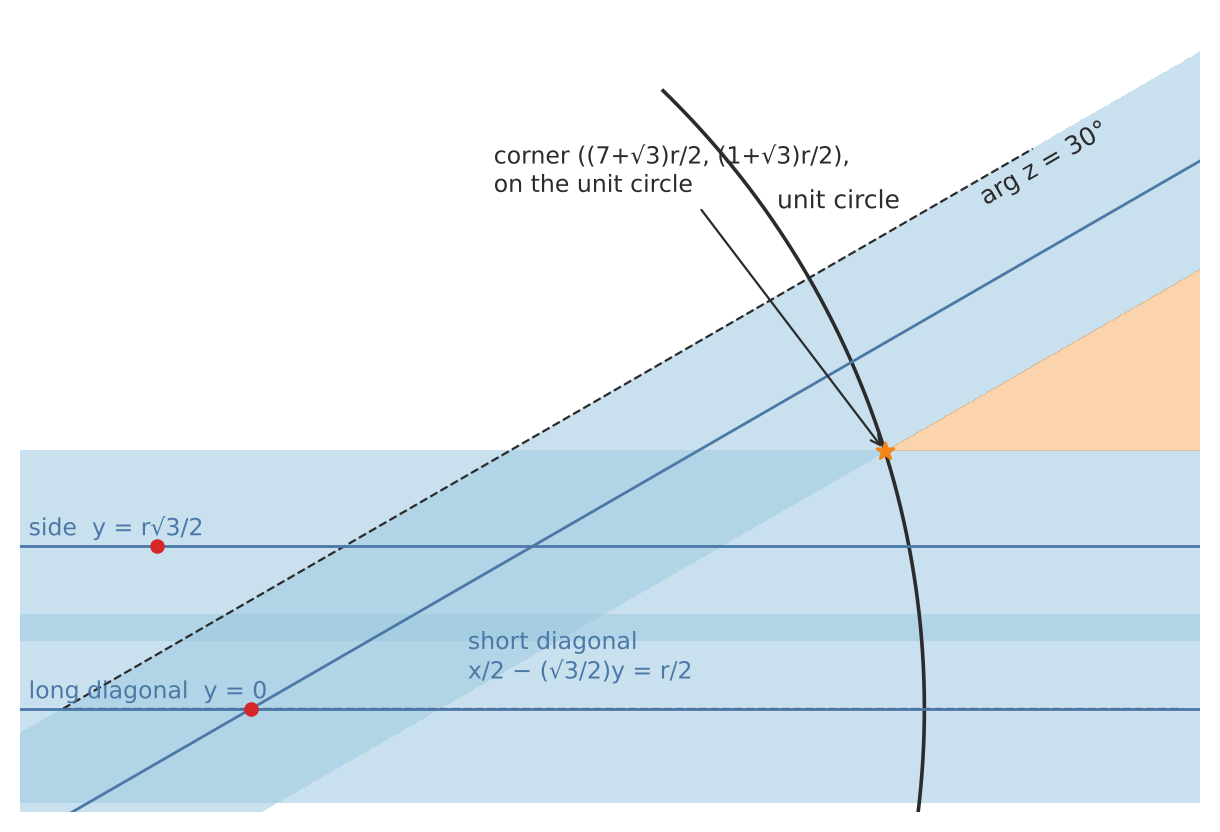
\includegraphics[width=0.62\textwidth]{figures/fig4_hexagon_sector.png}
\caption{The sector argument for the hexagon in Theorem~D. In the sector $0\le\arg z\le30^\circ$ (strips of half-width $r/2$ in blue), a point at
distance more than $r/2$ from the long diagonal $y=0$, the side $y=r\sqrt3/2$ and the short diagonal
$x/2-(\sqrt3/2)y=r/2$ lies in the orange region, whose corner $\bigl((7+\sqrt3)r/2,(1+\sqrt3)r/2\bigr)$ is on
the unit circle; so no point of the disc is that far from all $15$ lines.}\label{fig:hexsector}
\end{figure}

\begin{table}[ht]
\centering
\caption{The best cluster value $n^2\sin(\gamma_n/2)$. For $n=5,6$ the digits shown are certified by
Table~\ref{tab:gamma}; for $n\ge7$ they are the best configurations found (floating point; for $n\ge8$ the
searches did not converge).}\label{tab:clusters}
\small
\begin{tabular}{lcccccccc}
\toprule
$n$ & 5 & 6 & 7 & 8 & 9 & 10 & 11 & 12\\
\midrule
$n^2\sin(\gamma_n/2)$ & 4.261 & 3.975 & 4.051 & 4.044 & 4.045 & 4.185 & 4.095 & 4.274\\
\bottomrule
\end{tabular}
\end{table}

\begin{figure}[t]
\centering
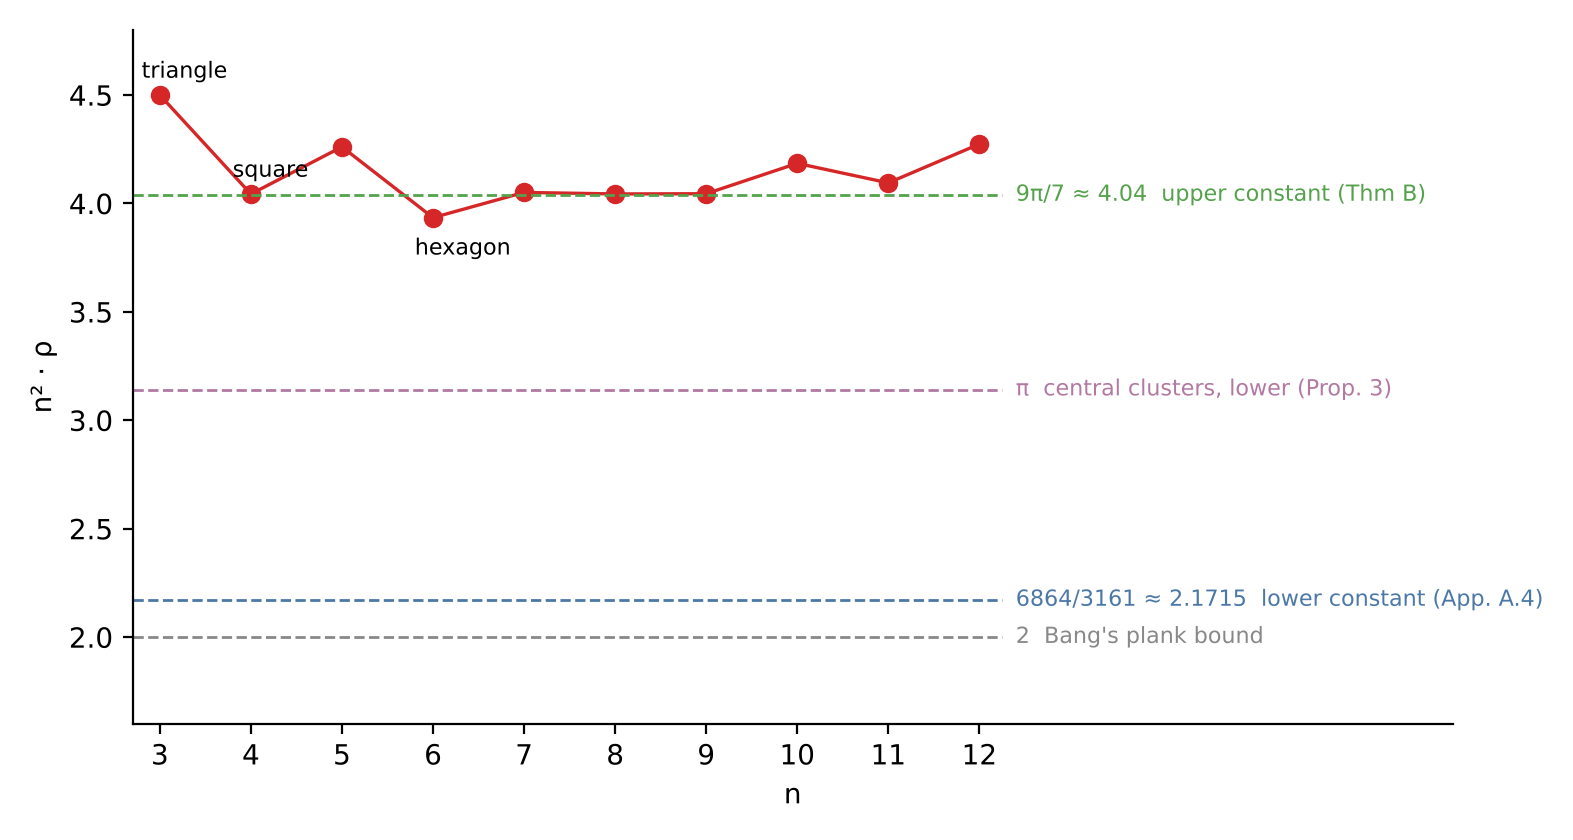
\includegraphics[width=0.8\textwidth]{figures/fig3_constants.png}
\caption{Best known $n^2\rho$ for $n=3,\dots,12$ (triangle, square and hexagon exact; the other values
are the best clusters found, floating point) against the asymptotic constants: Bang's $2$, the lower
constant $6864/3161\approx2.1715$ of Section~\ref{sec:A-sharp}, the cluster bound $\pi$ of Proposition~\ref{prop:clusters}, and the upper constant
$9\pi/7$ of Theorem~B.}\label{fig:constants}
\end{figure}

\section{Extensions}\label{sec:ext}

\subsection{Great hyperspheres through \texorpdfstring{$d$}{d} points}
\label{sec:D-spheres}

\begin{definition}\leavevmode
\begin{itemize}
  \item $\Sph^d\subset\R^{d+1}$ carries the angular metric. A linearly independent $d$-subset $F$ of a
    finite $P\subset\Sph^d$ spans the hyperplane $\spn(F)$ through $0$, and gives the great hypersphere
    $\Sph^d\cap\spn(F)$, at angular distance $\arcsin\abs{\ip{x}{\nu}}$ from $x\in\Sph^d$, $\nu$ a unit normal.
  \item For unit vectors $\nu_1,\dots,\nu_k$, $\rho(\nu)=\arcsin\max_{x\in\Sph^d}\min_j\abs{\ip{x}{\nu_j}}$ (the max is
    attained, and the signs of the $\nu_j$ do not matter). $\rho_S(P)$ is $\rho$ of the normals of the great
    hyperspheres of $P$ ($+\infty$ if there are none), and $\lambda_S^{(d)}(n)=\inf\rho_S(P)$ over $n$-point
    $P\subset\Sph^d$.
\end{itemize}
\end{definition}

\begin{proposition}\label{D:spheres}
For $d\ge2$ and $n>d$, $\pi/(2K)\le\lambda_S^{(d)}(n)\le\pi/(2p_d(n))$. (The Euclidean distance from $x\in\Sph^d$ to $\spn(F)$ is $\abs{\ip{x}{\nu}}$, the sine of the angular one; as
$\rho\le\pi/2$ and $\sin$ increases on $[0,\pi/2]$, the Euclidean covering radius of $P$ is $\sin\rho_S(P)$, and its
infimum lies between $\sin(\pi/(2K))$ and $\sin(\pi/(2p_d(n)))$.)
\end{proposition}

\begin{proof}
\textbf{Lower bound.} If $\rho=\rho_S(P)<\infty$, the closed angular $\rho$-neighbourhoods of the at most $K$
great hyperspheres are spherical segments of (angular) width $2\rho$ covering $\Sph^d$. By Glazyrin--Karasev--Polyanskii
\cite{GKP} (arXiv:2112.05382, Definition~1.14 and Corollary~1.15: if $\Sph^{m-1}$, $m\ge2$, is covered by spherical
segments, their angular widths sum to at least $\pi$), applied with $m=d+1$, $2\rho K\ge\pi$.

\textbf{Upper bound.} Let $N=p_d(n)$. The construction of Theorem~B (via Lemma~\ref{lem:B-lemma2-flats}) gives $n$-point
configurations $Q_s\subset\R^d$ ($s>0$) and a family $\mathcal F$ of $d$-subsets, affinely independent in
every $Q_s$, such that as $s\to0$ the hyperplane $\{y:\ip{\mu_F}{y}=c_F\}$ ($\abs{\mu_F}=1$) of each
$F\in\mathcal F$ converges to a hyperplane through $0$ containing a fixed $(d-2)$-subspace $L$: after a choice of
the sign of $(\mu_F,c_F)$, $\mu_F\to\mu_F^0$ and $c_F\to0$; and the limit normals $\mu_F^0$ lie in the plane $L^\perp$ with directions mod $\pi$
having largest gap $G\le\pi/N$. Lift $Q_s$ to $\Sph^d$ by $y\mapsto(y,1)/\abs{(y,1)}$; a $d$-subset is linearly
independent after the lift iff it was affinely independent, and the lift of $F$ spans the hyperplane with
unit normal $(\mu_F,-c_F)/\sqrt{1+c_F^2}\to(\mu_F^0,0)$.

For these limit normals and $x\in\Sph^d$, let $x_2$ be the component of $x$ in $L^\perp\times\{0\}$. Then
$\min_F\abs{\ip{x}{(\mu_F^0,0)}}=\min_F\abs{\ip{x_2}{\mu_F^0}}$. This is $0$ if $x_2=0$; otherwise it is
$\abs{x_2}\min_F\abs{\cos\angle(x_2,\mu_F^0)}=\abs{x_2}\min_F\sin\angle(x_2,\ell_F)\le\sin(G/2)$, where $\ell_F\subset L^\perp$ is
the line orthogonal to $\mu_F^0$: the lines $\ell_F$ also have largest gap $G$ mod $\pi$, so one is within $G/2$
of $x_2$, and $G/2\le\pi/2$ (gaps mod $\pi$ are at most $\pi$, $\mathcal F\ne\emptyset$); also $\abs{x_2}\le1$. Equality holds
for the unit $x=x_2$ at the middle of a largest gap. So the limit family has $\rho=G/2\le\pi/(2N)$. Finally,
$\sin\rho(\nu)$ is $1$-Lipschitz for the distance $\max_j\min_\pm\abs{\nu_j\mp\nu'_j}$ between families indexed alike
(since $\abs{\abs{\ip{x}{a}}-\abs{\ip{x}{b}}}\le\abs{a-b}$ for unit $x$) and $\arcsin$ is uniformly continuous,
so $\rho$ of the normals of the lifts of $F\in\mathcal F$ tends to $G/2$; the other great hyperspheres only
lower $\rho_S$. Hence $\lambda_S^{(d)}(n)\le\pi/(2N)$.
\end{proof}

The bounds of Proposition~\ref{D:spheres} coincide when $p_d(n)=\binom nd$, for example for
$n=d+1$ (take $\Z_{d+1}$) and for $(n,d)=(4,2),(6,3)$ (for the latter, the $20$ three-sums of $\{1,4,10,17,18,19\}\subset\Z_{20}$ are distinct); so the infimum is $\pi/(2(d+1))$ for $n=d+1$.

% ---------------------------------------------------------------------------
\subsection{Points anywhere: \texorpdfstring{$\mu_d(n)=\Theta(n^{-d})$}{mu\_d(n) = Theta(n\textasciicircum -d)} in every dimension, and \texorpdfstring{$\mu_d(d+1)=1/(d+1)$}{mu\_d(d+1) = 1/(d+1)}}
\label{sec:D-anywhere}

This proves the bounds for points anywhere in every dimension $d\ge2$.

\begin{definition}\leavevmode
\begin{itemize}
  \item For a finite $P\subset\R^d$ (anywhere, not only in
    $\ball^d$), $\mathcal{H}_P$ is the set of hyperplanes through $d$ affinely independent points
    of $P$, and
    \[
      \rho(P)=\max_{x\in\ball^d}\ \min_{H\in\mathcal{H}_P}\dist(x,H),
    \]
    with $\rho=\infty$ if $\mathcal{H}_P=\emptyset$.
  \item $\mu_d(n)=\inf\{\rho(P):P\subset\R^d,\ \abs{P}=n\}$, for $d\ge2$ and $n\ge d$.
  \item For a finite set $S$ of positive integers, $N_d(S)$ is the length of the longest run of
    consecutive integers all of which are sums of $d$ distinct elements of $S$.
    $N_d(n)=\max_{\abs{S}=n}N_d(S)$.
\end{itemize}
\end{definition}

\begin{proposition}\label{D:anywhere}
For $d\ge2$ and $n\ge d$:
\begin{enumerate}[label=(\roman*)]
  \item $1/\binom{n}{d}\le\mu_d(n)\le1/N_d(n)$.
  \item $\mu_d(d+1)=1/(d+1)$.
  \item $N_d(dq)\ge q^d$ for $q\ge2$. Since $\mu_d$ is non-increasing in $n$,
    \[
      d!\le\liminf n^d\mu_d(n)\le\limsup n^d\mu_d(n)\le d^d.
    \]
\end{enumerate}
\end{proposition}

\begin{proof}
\textbf{Lower bound.} Write the $k'\le\binom{n}{d}$ hyperplanes of $\mathcal{H}_P$ as
$\{x:\ip{x}{u_j}=m_j\}$ with $\abs{u_j}=1$. Lemma~\ref{lem:bang} does not need the points to lie in the ball.
The max defining $\rho(P)$ is attained ($\ball^d$ is compact), so the closed $\rho(P)$-slabs cover
$\ball^d$. Since $\abs{\ip{u_j}{v}}\le1$ for unit $v$,
$\rho k'\ge\rho\cdot\max_{\abs v=1}\sum_j\abs{\ip{u_j}{v}}\ge1$. So $\rho(P)\ge1/\binom{n}{d}$.

\begin{lemma}[Interpolation identity]\label{D:interp}
Let $t_1,\dots,t_d$ be distinct and nonzero, and let $p$ be the polynomial of degree $\le d-1$ with
$p(t_i)=1/t_i$. Then $p(0)=\sum_i1/t_i$.
\end{lemma}

\begin{proof}
The polynomial $1-t\,p(t)$ has degree $\le d$ and vanishes at every $t_i$, so
$1-t\,p(t)=c\prod_i(t-t_i)$. At $t=0$ this gives $c=1/\prod(-t_i)$. The coefficient of $t$ gives
$-p(0)=c\cdot(-1)^{d-1}e_{d-1}$, where $e_k$ are the elementary symmetric functions of the $t_i$. So
$p(0)=e_{d-1}/e_d=\sum1/t_i$.
\end{proof}

\textbf{Upper bound (i).} Let $S=\{u_1,\dots,u_n\}$ be distinct positive integers whose
$d$-distinct sums contain $c+1,\dots,c+N$. Put $t_i=1/u_i$, $\alpha=2/N$ and
$\beta=-1-\alpha c-\alpha/2$, so that $\alpha(c+j)+\beta=-1+(2j-1)/N$ for $j=1,\dots,N$. For $X>0$
let
\begin{equation*}
  p_i(X)=\bigl(Xt_i,\,Xt_i^2,\,\dots,\,Xt_i^{d-1},\,\alpha u_i+\beta\bigr)\in\R^d\qquad(i=1,\dots,n).
\end{equation*}

Write points of $\R^d$ as $(z,y)$ with $z\in\R^{d-1}$. Fix a $d$-set $F$, and let $p_F$ be the
interpolating polynomial of degree $\le d-1$ with $p_F(t_i)=\alpha/t_i+\beta$ for $i\in F$. Write
$p_F(t)=b_0+b_1t+\dots+b_{d-1}t^{d-1}$. Then the affine function
$g_F(z)=b_0+\sum_{k=1}^{d-1}(b_k/X)z_k$ satisfies $g_F(Xt_i,\dots,Xt_i^{d-1})=p_F(t_i)$, so its
graph contains $p_i(X)$ for $i\in F$.

The points $p_i(X)$, $i\in F$, are affinely independent. Their first $d-1$ coordinates are
$X\cdot(t_i,\dots,t_i^{d-1})$, which are affinely independent by Vandermonde. So the graph of $g_F$
is the hyperplane $H_F(X)$ through them, and every $d$-set is independent.

By the identity (Lemma~\ref{D:interp}), $b_0=p_F(0)=\alpha\sum_{i\in F}u_i+\beta$. The $b_k$ do not
depend on $X$. So as $X\to\infty$, $H_F(X)$ converges (unit normal and offset) to the horizontal
hyperplane $\{y=\alpha\sum_{i\in F}u_i+\beta\}$.

The covering radius of a fixed finite list of hyperplanes is continuous in their normals and
offsets: for $\abs{x}\le1$, $\abs{\dist(x,H)-\dist(x,H')}\le\abs{n-n'}+\abs{c-c'}$, and max-min
preserves this bound. So $\rho(P(X))$ tends to the covering radius of the limit list. That list
contains the horizontal hyperplanes at heights $-1+(2j-1)/N$, $j=1,\dots,N$, whose $1/N$-slabs cover
$\ball^d$. Hence $\mu_d(n)\le\lim\rho(P(X))\le1/N$.

\textbf{(ii)} Take $S=\{1,\dots,d+1\}$. Its $d$-distinct sums are $T-s$ for $s\in S$, where
$T=\sum S$. These are $d+1$ consecutive integers, so $N_d(d+1)\ge d+1$. Together with the lower
bound $1/\binom{d+1}{d}$, $\mu_d(d+1)=1/(d+1)$.

\textbf{(iii)} Let $L=q^d$ and
\[
  S=\bigcup_{j=0}^{d-1}\{aq^j+jL+1:0\le a<q\}:
\]
$d$ blocks of $q$ elements, $n=dq$. Elements within a block are distinct since $q^j\ge1$, and the
blocks are disjoint, since (using $(q-1)q^j+1\le q^d$) block $j$ lies in
$[jL+1,\,jL+1+(q-1)q^{d-1}]\subset[jL+1,\,(j+1)L]$. Choosing one element from each block gives
distinct elements with sum $\sum_ja_jq^j+\sum_j(jL+1)$. As $(a_0,\dots,a_{d-1})$ ranges over
$\{0,\dots,q-1\}^d$, $\sum a_jq^j$ takes all values $0,\dots,q^d-1$. So $N_d(dq)\ge q^d$ and
$\mu_d(dq)\le q^{-d}$.

Adding a point never removes a hyperplane, so $\mu_d$ is non-increasing in $n$. For
$dq\le n<d(q+1)$, $n^d\mu_d(n)\le(d(q+1))^d/q^d\to d^d$. The liminf bound is
$n^d/\binom{n}{d}\to d!$.
\end{proof}

\begin{lemma}[The plane]\label{D:N2}
$N_2(n)\ge\lfloor n^2/4\rfloor$ for $n\ge2$, so $\mu_2(n)\le1/\lfloor n^2/4\rfloor$. Moreover $\mu_2(3)=1/3$
and $\mu_2(4)=1/6$.
\end{lemma}

\begin{proof}
Let $a=\lfloor n/2\rfloor$, $A=\{1,\dots,a\}$ and $B=\{2a,3a,\dots,(n-a+1)a\}$: $n$ distinct positive
integers. The sums $i+ja$ ($1\le i\le a$, $2\le j\le n-a+1$) of distinct elements fill the interval
$[2a+1,(n-a+2)a]$, which contains $a(n-a)=\lfloor n^2/4\rfloor$ integers. With
Proposition~\ref{D:anywhere}(i) this gives $\mu_2(n)\le1/\lfloor n^2/4\rfloor$. $\mu_2(3)=1/3$ is
Proposition~\ref{D:anywhere}(ii) with $d=2$. The pair sums of
$\{1,2,3,5\}$ are $3,\dots,8$, so $1/6=1/\binom42\le\mu_2(4)\le1/N_2(4)\le1/6$.
\end{proof}

% ---------------------------------------------------------------------------
\subsection{Flats through \texorpdfstring{$j+1$}{j+1} points: \texorpdfstring{$\lambda_d^{(j)}(n)=\Theta(n^{-(j+1)/(d-j)})$}{lambda = Theta(n\textasciicircum(-(j+1)/(d-j)))} for every \texorpdfstring{$1\le j\le d-1$}{1 <= j <= d-1}}
\label{sec:D-flats}

For $j=1$ (lines) this section proves the tube bound $k\rho^{d-1}\ge1$ and, in $\ball^3$,
$\sqrt2\le\liminf n\lambda\le\limsup n\lambda\le6\sqrt2$. For $j=d-1$ (hyperplanes) it recovers the
order $n^{-d}$, with weaker constants than Corollary~C.

\begin{definition}\leavevmode
\begin{itemize}
  \item $d\ge2$ and $1\le j\le d-1$. Put $m=d-j+1\ge2$.
    $\Sph^{k-1}$ is the unit sphere of $\R^k$, $\kappa_k=\pi^{k/2}/\Gamma(k/2+1)$ and
    $\abs{\Sph^{k-1}}=2\pi^{k/2}/\Gamma(k/2)$.
  \item A $j$-flat is an affine $j$-dimensional subspace. For $P\subset\ball^d$ with $n\ge j+1$
    points, $\mathcal{F}_P$ is the set of $j$-flats spanned by affinely independent
    $(j+1)$-subsets of $P$, so $\abs{\mathcal{F}_P}\le K=\binom{n}{j+1}$. Put
    \[
      \rho(P)=\max_{x\in\ball^d}\ \min_{F\in\mathcal{F}_P}\dist(x,F)\quad(=\infty\text{ if }\mathcal{F}_P=\emptyset),
    \]
    and $\lambda_d^{(j)}(n)=\inf\{\rho(P):P\subset\ball^d,\ \abs{P}=n\}$.
  \item $\delta(W)$, for a finite set $W\subset\R^m\setminus\{0\}$, is as in Section~\ref{sec:B-lemma2}.
\end{itemize}
\end{definition}

\begin{proposition}[Lower bound]\label{D:M1}
If the $\rho$-neighbourhoods of $K$ $j$-flats cover $\ball^d$, then $K\rho^{d-j}\ge c(d,j)$, where
\begin{equation*}
  c(d,1)=1,\qquad c(d,j)=\frac{\Gamma(j/2)\,\Gamma((d-j)/2+1)}{\Gamma(d/2)}\quad(j\ge2).
\end{equation*}
Hence $\binom{n}{j+1}\cdot\lambda_d^{(j)}(n)^{d-j}\ge c(d,j)$.
\end{proposition}

For $j=1$ this is the tube bound $k\rho^{d-1}\ge1$ for $k$ lines: the density $(1-|x|^2)^{-1/2}$ integrates to exactly $\pi$ along every line, and the bound is the ellipsoid case of Bezdek and Litvak's theorem on covering convex bodies by cylinders \cite{BL}, proved there with the same density (for $d=2$ it is Bang's bound for the disc). For $(d,j)=(3,2)$ it is the plank bound $K\rho\ge1$. For
$j\ge2$ it beats the volume bound $\kappa_d/(\kappa_j\kappa_{d-j})$ by the factor $d/j$.

\begin{proof}
For $0\le a<1$ let $f_a(x)=(1-\abs{x}^2)^{-a}$ on the open ball.
\begin{enumerate}[label=(\alph*)]
  \item \textbf{A flat.} Let $F$ be a $j$-flat at distance $h<1$ from $0$, and $R=\sqrt{1-h^2}$.
    Then
    \[
      \int_{F\cap\ball^d}f_a=\abs{\Sph^{j-1}}\int_0^Rr^{j-1}(R^2-r^2)^{-a}\,dr
      =R^{j-2a}\cdot\tfrac12\abs{\Sph^{j-1}}\,B(j/2,1-a).
    \]
    If $a\le j/2$, this is at most $I_j(a):=\frac12\abs{\Sph^{j-1}}\,B(j/2,1-a)$, its value at
    $h=0$. Flats with $h\ge1$ miss the open ball.
  \item \textbf{The ball.} $\int_{\ball^d}f_a=\frac12\abs{\Sph^{d-1}}\,B(d/2,1-a)$.
  \item \textbf{A neighbourhood.} The $\rho$-neighbourhood of $F$ is the union of the parallel flats
    $F+w$, for $w$ in the $(d-j)$-dimensional orthogonal complement of the direction of $F$ with
    $\abs{w}\le\rho$. By Fubini and (a), its $f_a$-mass is at most $\kappa_{d-j}\rho^{d-j}I_j(a)$.
  \item \textbf{Covering.} $K\kappa_{d-j}\rho^{d-j}I_j(a)\ge\frac12\abs{\Sph^{d-1}}\,B(d/2,1-a)$.
    Simplifying with $B(x,y)=\Gamma(x)\Gamma(y)/\allowbreak\Gamma(x+y)$:
    \begin{equation*}
      K\rho^{d-j}\ge c_a:=\frac{\Gamma(j/2+1-a)\,\Gamma((d-j)/2+1)}{\Gamma(d/2+1-a)},
    \end{equation*}
    for every $a<1$ with $a\le j/2$.
    For $j=1$ take $a=\frac12$: $c_{1/2}=1$. For $j\ge2$ let $a\uparrow1$: $c_a\to c(d,j)$. The bound
    holds for every $a<1$, so it holds in the limit. With $a=0$,
    $c_0=\kappa_d/(\kappa_j\kappa_{d-j})$ is the volume bound, and $c(d,j)/c_0=d/j$ for
    $j\ge2$.\qedhere
\end{enumerate}
\end{proof}

\begin{lemma}[Flat clusters through a $(j-1)$-space]\label{D:M2}
Write $\R^d=\R^{j-1}\times\R^m$. Let $\tau_0<\dots<\tau_j$ be reals,
$t_r=\eta\cdot(\tau_r,\tau_r^2,\dots,\tau_r^{j-1})\in\R^{j-1}$ (empty if $j=1$) with $\eta>0$ (a
scale),
and $c_r=1/\prod_{k\ne r}(\tau_r-\tau_k)$. Then $\sum_rc_r=0$ and $\sum_rc_rt_r=0$, and $c$ spans
the affine dependencies of $t_0,\dots,t_j$. For $a_r\in\R^m$ with $w=\sum_rc_ra_r\ne0$, and $s>0$,
the points $q_r=(t_r,sa_r)$ are affinely independent. As $s\to0$, their $j$-flat converges (in the
sense that $x\mapsto\dist(x,\cdot)$ converges uniformly on $\ball^d$) to the linear subspace
$L_w=(\R^{j-1}\times\{0\})\oplus\R(0,w)$.
\end{lemma}

\begin{proof}
\emph{The dependency.} The $j$-th divided difference $\sum_rc_rp(\tau_r)$ of a polynomial of degree
$<j$ vanishes. So $\sum_rc_rp(\tau_r)=0$ for $p=1,\tau,\dots,\tau^{j-1}$, which gives $\sum c_r=0$
and $\sum c_rt_r=0$. The $t_r$ affinely span $\R^{j-1}$: any $j$ of them have Vandermonde determinant
$\ne0$. So the dependency space is one-dimensional and spanned by $c$. The rest is
Lemma~\ref{lem:B-lemma2-flats}(i) and~(ii), applied to these $t_r$, $c$ and $a_r$.
\end{proof}

For linear $L_w$ and any $x$, $\dist(x,L_w)=\abs{x_\perp}\sin\angle(x_\perp,\R w)$, where $x_\perp$
is the $\R^m$-component (read as $0$ when $x_\perp=0$). Hence
\begin{equation*}
  \max_{x\in\ball^d}\ \min_{w\in W}\dist(x,L_w)=\sin\delta(W).
\end{equation*}

\begin{proposition}[Construction]\label{D:M3}
Let $M\ge2$ and $N=M^{j+1}$, and assume $N-1\ge(2/\pi)\sqrt{m-1}$, so that
$\theta:=\sqrt{m-1}/(N-1)\le\pi/2$. Then
\begin{equation*}
  \lambda_d^{(j)}\bigl(m(j+1)M^{m-1}\bigr)\le\sin\theta.
\end{equation*}
Adding a point keeps every flat already spanned, so $\lambda$ is non-increasing in $n$; hence
\begin{equation*}
  \limsup_n n^{(j+1)/(d-j)}\lambda_d^{(j)}(n)\le\sqrt{d-j}\cdot\bigl((d-j+1)(j+1)\bigr)^{(j+1)/(d-j)}.
\end{equation*}
\end{proposition}

For $j=1$, $d=3$ this is $6\sqrt2$. For $j=d-1$ it is $(2d)^d$.

\begin{proof}
\emph{Construction (one block).} Take $\tau_r=r$ ($r=0,\dots,j$), and $t_r$, $c_r$ as in
Lemma~\ref{D:M2}. Let $G=\{0,\dots,M-1\}^{m-1}$, $h=(N-1)/2$ and $e=(1,\dots,1)\in\R^{m-1}$. Group
$r$ consists of the points $(t_r,s\cdot b/c_r)$, where $b$ runs over
\begin{itemize}
  \item $r=0$: $B_0=\{(g-h\cdot e,\,h):g\in G\}\subset\R^{m-1}\times\R$;
  \item $r\ge1$: $B_r=\{(M^rg,\,0):g\in G\}$.
\end{itemize}
Each group has $M^{m-1}$ points, distinct because the $b$'s are distinct. Groups are distinct
because their $t_r$ differ. For $j=1$ there is no $t$; then $c_0=-1$ and $c_1=1$, group $0$ has last
coordinate $-s\cdot h\ne0$ and group $1$ has last coordinate $0$, so the groups are distinct too.

\emph{Transversal sets.} Take one point from each group, $F=\{(t_r,sb_r/c_r)\}$. Then
\[
  w_F=\sum_rc_r(b_r/c_r)=\sum_rb_r=(g_0+Mg_1+\dots+M^jg_j-h\cdot e,\,h).
\]
By base-$M$ digits, $g_0+\dots+M^jg_j$ runs over $\{0,\dots,N-1\}^{m-1}$. So the set $W$ of all
$w_F$ is $\{(x,h):x\in\{-h,-h+1,\dots,h\}^{m-1}\}$, and $w_F\ne0$. By Lemma~\ref{D:M2}, these flats
converge to $L_{w_F}$.

\emph{Covering one chart.} Let $x\in\Sph^{m-1}$ with $\abs{x_i}\le x_m$ for $i<m$. Then $x$ is a
positive multiple of $(p,1)$ with $p\in[-1,1]^{m-1}$. Writing $w=(z,h)$, the points
$w/h=(z/h,1)$ have $z/h$ on a grid of spacing $1/h$ covering $[-1,1]^{m-1}$, so some has
$\abs{p-z/h}\le\sqrt{m-1}/(2h)=\sqrt{m-1}/(N-1)$. By the gnomonic inequality
$\angle((p,1),(p',1))\le\abs{p-p'}$ for $p,p'\in\R^{m-1}$, the angle is at most $\sqrt{m-1}/(N-1)$.
(Proof: the path $P(s)=(p+s(p'-p),1)$, $s\in[0,1]$, has $\abs{P(s)}\ge1$; the angle is at most the
length of the spherical path $P/\abs P$, and $\abs{(P/\abs P)'}\le\abs{P'}/\abs P$, so the length is at
most $\int_0^1\abs{P'(s)}/\abs{P(s)}\,ds\le\abs{p'-p}$.)

\emph{All directions: $m$ blocks.} For $\sigma$ the cyclic permutation of the $m$ coordinates of
$\R^m$, block $i$ ($i=0,\dots,m-1$) applies $\sigma^i$ to the $\R^m$-components of block $0$, and
adds $s\cdot v_i$ to them, with $v_i\in\R^m$ chosen so that all points of all blocks are distinct
(this excludes finitely many affine conditions, so generic $v_i$ work). The translation does not
change $w_F$, since $\sum c_r=0$. Every $x\in\Sph^{m-1}$ is $\pm\sigma^i$ of a vector in the chart
above for some $i$. So $\delta(W_{\mathrm{all}})\le\sqrt{m-1}/(N-1)$, with $n=m(j+1)M^{m-1}$ points
in total.

\emph{Conclusion.} Take $\eta$ small enough that $\abs{t_r}<\frac12$, and $s$ small enough that all
points lie in $\ball^d$. Let $\mathcal{F}_s$ be the family of $j$-flats spanned by the transversal
sets of all blocks. Then $\rho(P_s)\le\max_x\min_{F\in\mathcal{F}_s}\dist(x,F)$, because extra flats
only lower $\rho$. By Lemma~\ref{D:M2} and uniform convergence, the right side tends to
$\sin\delta(W_{\mathrm{all}})\le\sin\theta$, using $\theta\le\pi/2$ (the hypothesis) and $\sin$
increasing on $[0,\pi/2]$. Without the hypothesis the bound can fail: for $(d,j,M)=(90,1,2)$,
$\theta>\pi$ and $\sin\theta<0$. For the limsup, put
$M=\bigl\lfloor(n/(m(j+1)))^{1/(m-1)}\bigr\rfloor$, which satisfies the hypothesis for large $n$, and
use monotonicity in $n$.
\end{proof}

\begin{corollary}\label{D:M4}
For all $d\ge2$ and $1\le j\le d-1$, $\lambda_d^{(j)}(n)=\Theta(n^{-(j+1)/(d-j)})$, with
\begin{align*}
  \bigl((j+1)!\cdot c(d,j)\bigr)^{1/(d-j)}&\le\liminf n^{(j+1)/(d-j)}\lambda\\
  &\le\limsup n^{(j+1)/(d-j)}\lambda\le\sqrt{d-j}\cdot\bigl((d-j+1)(j+1)\bigr)^{(j+1)/(d-j)}.
\end{align*}
\end{corollary}

The lower constant comes from Proposition~\ref{D:M1} with $\binom{n}{j+1}\sim n^{j+1}/(j+1)!$. For
example, for planes through triples in $\ball^4$ ($d=4$, $j=2$):
$\sqrt6\approx2.45\le\liminf n^{3/2}\lambda\le\limsup n^{3/2}\lambda\le27\sqrt2\approx38.2$.


\begin{remark}[Lines through the centre of $\ball^3$]
If $k$ lines through $0$ have covering radius $\rho=\max_{x\in\ball^3}\min_\ell\dist(x,\ell)<1$, each $\rho$-tube meets $\Sph^2$ in two antipodal
caps of area $2\pi\bigl(1-\sqrt{1-\rho^2}\bigr)$, and the caps cover $\Sph^2$. So
$k\bigl(1-\sqrt{1-\rho^2}\bigr)\ge1$, that is $k\rho^2\ge1+\sqrt{1-\rho^2}\to2$, against $k\rho^2\ge1$
in general. This is the analogue for lines of the cost $\pi$ against $2$ of Proposition~\ref{prop:clusters}.
\end{remark}

\subsection{Every convex body: \texorpdfstring{$\lambda_d(n;\Omega)=\Theta(n^{-d})$}{lambda\_d(n;Omega) = Theta(n\textasciicircum -d)} and \texorpdfstring{$\mu_d(d+1;\Omega)=w(\Omega)/(2(d+1))$}{mu\_d(d+1;Omega) = w(Omega)/(2(d+1))}}
\label{sec:D-convex}\label{sec:convex}

This generalizes the order $\lambda_d(n)=\Theta(n^{-d})$ (Corollary~C) and the points-anywhere results
from the unit ball to every convex body. It uses only Bang's plank theorem, Theorem~B's construction with
Lemma~\ref{lem:B-lemma2-flats}, and the construction of Section~\ref{sec:D-anywhere}. Theorem~A's strict gain over Bang is not
generalized (its measure is specific to the ball).

\begin{definition}\leavevmode
\begin{itemize}
  \item A convex body $\Omega\subset\R^d$ ($d\ge2$) is a compact convex set with nonempty interior.
  \item $w(\Omega)$ is its minimal width: the least distance between two parallel supporting hyperplanes. It
    is attained, since the width in direction $u$ is continuous on the compact sphere $\Sph^{d-1}$.
  \item $R(\Omega)=\min_{c\in\R^d}\max_{x\in \Omega}\abs{x-c}$ is its circumradius.
  \item For a finite $P\subset\R^d$, $H_P$ is the set of hyperplanes through $d$ affinely independent
    points of $P$, and $\rho_\Omega(P)=\max_{x\in \Omega}\min_{H\in H_P}\dist(x,H)$ ($=\infty$ if $H_P=\emptyset$).
    The max is attained ($\Omega$ is compact).
  \item $\lambda_d(n;\Omega)=\inf\{\rho_\Omega(P):P\subset \Omega,\ |P|=n\}$ and
    $\mu_d(n;\Omega)=\inf\{\rho_\Omega(P):P\subset\R^d,\ |P|=n\}$. For $\Omega=\ball^d$ these are $\lambda_d(n)$ and
    $\mu_d(n)$.
  \item $p_d(n)$, $\sigma_d$ and $N_d(n)$ are as in Theorem~B and Section~\ref{sec:D-anywhere}.
\end{itemize}
\end{definition}

The order of every covering radius in this paper extends; the sharp results do not.

\begin{center}
\small
\begin{tabular}{p{3.4cm}p{5.2cm}p{5.6cm}}
\toprule
Result & Unit ball & Convex body $\Omega$\\
\midrule
Order of $\lambda_d(n)$ & $\ell_d\le\liminf n^d\lambda_d(n)$ (Corollary~C), $\limsup\le\pi/(2\sigma_d)$ &
$d!\,w(\Omega)/2\le\liminf n^d\lambda_d(n;\Omega)$, $\limsup\le\pi R(\Omega)/(2\sigma_d)$\\
Points anywhere, $n=d+1$ & $\mu_d(d+1)=1/(d+1)$ & $\mu_d(d+1;\Omega)=w(\Omega)/(2(d+1))$\\
Strict gain over Bang (Theorem~A, Corollary~1) & yes & open\\
\bottomrule
\end{tabular}
\end{center}

\paragraph{Bang's plank theorem} (Verreault's survey \cite{Verreault},
Theorem~2.2, quoted from the arXiv v2 HTML): ``Let $C\subset\R^d$ be a convex body covered by $n$ planks
$P_j$, $j=1,\dots,n$. Then $w(P_1)+\dots+w(P_n)\ge w(C)$.'' There a (closed) plank is ``the closed set
of points between two parallel hyperplanes'', its width is the distance between them, and $w(C)$ is the
minimal width. The survey attributes the theorem to Bang (1950; simplified 1951).

\begin{proposition}\label{D:convex}
Let $\Omega\subset\R^d$ be a convex body, $d\ge2$.
\begin{enumerate}[label=(\roman*)]
  \item For $n\ge d$: $\mu_d(n;\Omega)\ge w(\Omega)/(2\binom nd)$, and so $\lambda_d(n;\Omega)\ge w(\Omega)/(2\binom nd)$.
  \item For $n\ge d+1$: $\lambda_d(n;\Omega)\le R(\Omega)\sin(\pi/(2p_d(n)))$.
  \item For $n\ge d$: $\mu_d(n;\Omega)\le w(\Omega)/(2N_d(n))$. Hence $\mu_d(d+1;\Omega)=w(\Omega)/(2(d+1))$ and
    $d!\,w(\Omega)/2\le\liminf n^d\mu_d(n;\Omega)\le\limsup n^d\mu_d(n;\Omega)\le d^d\,w(\Omega)/2$.
  \item $\lambda_d(n;\Omega)=\Theta(n^{-d})$:
    $d!\,w(\Omega)/2\le\liminf n^d\lambda_d(n;\Omega)\le\limsup n^d\lambda_d(n;\Omega)\le\pi R(\Omega)/(2\sigma_d)$.
\end{enumerate}
\end{proposition}

For $\Omega=\ball^d$ ($w=2$, $R=1$) these are the bounds $1/\binom nd\le\lambda_d(n)\le\sin(\pi/2p_d(n))$,
$\mu_d(d+1)=1/(d+1)$, and so on.

\begin{proof}
\textbf{(i)} Let $P\subset\R^d$ with $|P|=n$ and $\rho=\rho_\Omega(P)<\infty$. Then $\rho>0$, since finitely
many hyperplanes cannot cover $\Omega$, which has nonempty interior. Since the max defining $\rho$ is attained,
every $x\in \Omega$ is within $\rho$ of some $H\in H_P$, so the closed planks $\{x:\dist(x,H)\le\rho\}$,
$H\in H_P$, of width $2\rho$ cover $\Omega$. There are at most $\binom nd$ of them. By Bang's plank theorem,
$\binom nd\cdot2\rho\ge w(\Omega)$. Taking the infimum over $P$ gives the bound for $\mu_d(n;\Omega)$, and
$\lambda_d(n;\Omega)\ge\mu_d(n;\Omega)$ since the infimum is over a smaller set.

\textbf{(ii)} \emph{The circumcentre.} $c\mapsto f(c)=\max_{x\in \Omega}\abs{x-c}$ is $1$-Lipschitz and tends
to $\infty$, so its minimum $R(\Omega)$ is attained at some $c^*$. Then $c^*\in \Omega$: otherwise let $y$ be the
nearest point of $\Omega$ to $c^*$; for every $x\in \Omega$, $\ip{x-y}{c^*-y}\le0$, so
$\abs{x-c^*}^2=\abs{x-y}^2+\abs{y-c^*}^2-2\ip{x-y}{c^*-y}>\abs{x-y}^2$, and $f(y)<f(c^*)$, a
contradiction. Since $\Omega$ is the closure of its interior and $f$ is continuous,
$\inf_{c\in\operatorname{int}\Omega}f(c)=R(\Omega)$. So it suffices to show
$\lambda_d(n;\Omega)\le f(z)\sin(\pi/(2N))$ for every $z\in\operatorname{int}\Omega$, where $N=p_d(n)$.

\emph{The construction.} Fix $z\in\operatorname{int}\Omega$ and $\eta>0$ with $B(z,\eta)\subset \Omega$. Take
$S\subset\Z_N$, $|S|=n$, as in Theorem~B, and, as in its proof, $\theta_j$, $\tau_j=-\cot\theta_j$ and
\[
  q_j(r)=\bigl(\kappa\cdot(\tau_j,\dots,\tau_j^{d-2}),\ r/(i-\tau_j)\bigr)\in\R^{d-2}\times\mathbb C=\R^d
  \qquad(j=1,\dots,n;\ 0<r\le1),
\]
with the $n$ values $\tau_j$ distinct. These $n$ points are distinct (their last components
$r/(i-\tau_j)$ are distinct). For every $d$-subset $F$, the $d$ points
$t_j=\kappa(\tau_j,\dots,\tau_j^{d-2})$, $j\in F$, affinely span $\R^{d-2}$ (Vandermonde), with dependency
$c_j=1/\prod_{k\in F,k\ne j}(\tau_j-\tau_k)$, and $w_F=\sum_{j\in F}c_j/(i-\tau_j)\ne0$. So
Lemma~\ref{lem:B-lemma2-flats} (with $j=d-1$, $m=2$, $a_j=1/(i-\tau_j)$, $s=r$) applies: the
points $q_j(r)$, $j\in F$, are affinely independent, and their hyperplane $H_F(r)$ satisfies
$\dist(\cdot,H_F(r))\to\dist(\cdot,L_F)$ as $r\to0$, where $L_F=(\R^{d-2}\times\{0\})\oplus\R(0,w_F)$.

The convergence is uniform on every ball $B(0,\mathcal R)$, not only on $\ball^d$: in the proof of
Lemma~\ref{lem:B-lemma2-flats}(ii), for $\abs y\le\mathcal R$,
$\abs{(I-\Pi_s)(y-q)-(I-\Pi)(y-q_0)}\le\norm{\Pi_s-\Pi}(\mathcal R+\abs q)+\abs{q-q_0}$, with
$q=q_{i_0}$, $q_0=(t_{i_0},0)$, using $\norm{I-\Pi}\le1$.

By the proof of Theorem~B, the directions of the $w_F$ mod $\pi$, over all $d$-subsets $F$, are $N$
equally spaced ones, so their largest gap mod $\pi$ is $G=\pi/N$.

\emph{Placing it in $\Omega$.} Let $M_0=\sup_{j,\,0<r\le1}\abs{q_j(r)}<\infty$ and $\zeta=\eta/M_0$. The
points $P_j(r)=z+\zeta q_j(r)$ lie in $B(z,\eta)\subset \Omega$, are distinct, and every $d$ of them are
affinely independent, with hyperplane $z+\zeta H_F(r)$. For $x\in \Omega$,
$\dist(x,z+\zeta H_F(r))=\zeta\dist((x-z)/\zeta,H_F(r))$, and $(x-z)/\zeta$ ranges over a bounded set
as $x$ ranges over $\Omega$. So, uniformly in $x\in \Omega$,
$\dist(x,z+\zeta H_F(r))\to\zeta\dist((x-z)/\zeta,L_F)=\dist(x-z,L_F)$, since $L_F$ is a linear
subspace.

\emph{The limit.} A max over $x\in \Omega$ of a min of finitely many functions moves by at most $\eta'$ when
each function moves by at most $\eta'$ uniformly. So
$\rho_\Omega(\{P_j(r)\})\to\max_{x\in \Omega}\min_F\dist(x-z,L_F)$. For $y=x-z$ write
$y=(y_1,y_2)\in\R^{d-2}\times\R^2$. Then $\dist(y,L_F)=\abs{y_2}\sin\angle(y_2,\R w_F)$ ($0$ if
$y_2=0$). Every direction in $\R^2$ is within $G/2=\pi/(2N)\le\pi/2$ of some line $\R w_F$, and $\sin$
increases on $[0,\pi/2]$, so $\min_F\dist(y,L_F)\le\abs{y_2}\sin(\pi/(2N))\le\abs{x-z}\sin(\pi/(2N))$.
Hence $\lambda_d(n;\Omega)\le\lim_{r\to0}\rho_\Omega(\{P_j(r)\})\le f(z)\sin(\pi/(2N))$.

\textbf{(iii)} Choose a unit vector $e$ with width $w(\Omega)$ in direction $e$, and $h_0$ with
$\Omega\subset\{h_0\le\ip xe\le h_0+w(\Omega)\}$. After a rotation and translation, which change neither $\rho_\Omega$
nor the widths, $e=e_d$ and $h_0=0$. Let $N=N_d(n)$ and $S=\{u_1,\dots,u_n\}$ be distinct positive
integers whose $d$-distinct sums contain $c_0+1,\dots,c_0+N$. Apply the construction of
Section~\ref{sec:D-anywhere} (upper bound (i)) with $\alpha=w(\Omega)/N$ and $\beta=-\alpha c_0-\alpha/2$ in
place of $\alpha=2/N$ and $\beta=-1-\alpha c_0-\alpha/2$:
\begin{itemize}
  \item the points $p_i(X)=(Xt_i,\dots,Xt_i^{d-1},\alpha u_i+\beta)$, $t_i=1/u_i$, have every $d$-subset
    affinely independent;
  \item the hyperplane $H_F(X)$ of a $d$-subset $F$ converges in unit normal and offset, as $X\to\infty$,
    to the horizontal hyperplane $\{x_d=\alpha\sum_{i\in F}u_i+\beta\}$. (The proof there works for any
    $\alpha,\beta$: the hyperplane is the graph of $g_F(z)=b_0+\sum_k(b_k/X)z_k$ with
    $b_0=\alpha\sum_{i\in F}u_i+\beta$, and the $b_k$ do not depend on $X$.)
\end{itemize}
The limit list contains the hyperplanes $\{x_d=(j-\frac12)w(\Omega)/N\}$, $j=1,\dots,N$, whose closed
$w(\Omega)/(2N)$-slabs cover $\{0\le x_d\le w(\Omega)\}\supset \Omega$. For $x\in \Omega$, with
$\mathcal R=\max_{x\in \Omega}\abs x$,
\[
  \abs{\dist(x,H)-\dist(x,H')}\le\mathcal R\abs{n-n'}+\abs{o-o'}
\]
for hyperplanes with unit normals $n,n'$ and offsets $o,o'$, and a max-min moves by at most the largest such
change. So $\rho_\Omega(P(X))$ tends to the covering radius of the limit list over $\Omega$, which is at most
$w(\Omega)/(2N)$. Hence $\mu_d(n;\Omega)\le w(\Omega)/(2N_d(n))$.

For $n=d+1$, $N_d(d+1)\ge d+1$ (Section~\ref{sec:D-anywhere}), and (i) gives the matching lower bound
$w(\Omega)/(2\binom{d+1}d)=w(\Omega)/(2(d+1))$. For the limits: $N_d(dq)\ge q^d$ (Section~\ref{sec:D-anywhere},
for $q\ge2$; trivially for $q=1$), and $\mu_d(n;\Omega)$ is non-increasing in $n$ (adding a point keeps every
hyperplane), so for $dq\le n<d(q+1)$, $n^d\mu_d(n;\Omega)\le(d(q+1))^dw(\Omega)/(2q^d)\to d^dw(\Omega)/2$; and
$n^dw(\Omega)/(2\binom nd)\to d!\,w(\Omega)/2$.

\textbf{(iv)} The lower bound is (i) with $n^d/\binom nd\to d!$. For the upper bound, $\sin x\le x$
gives $n^d\lambda_d(n;\Omega)\le R(\Omega)\pi n^d/(2p_d(n))$, and $p_d(n)/n^d\to\sigma_d>0$ (Theorem~B and
Corollary~C), so $\limsup n^d\lambda_d(n;\Omega)\le\pi R(\Omega)/(2\sigma_d)$.
\end{proof}

\begin{remark}
The two constants in (iv) depend on $\Omega$ through $w(\Omega)$ and $R(\Omega)$ separately, and their ratio
$(\pi/(d!\,\sigma_d))R(\Omega)/w(\Omega)$ is not bounded over convex bodies: a $1\times\eps$ rectangle has
$w=\eps$ and $R\approx\frac12$. For such thin bodies the construction in (ii), a pencil through a common
$(d-2)$-flat, is far from the lower bound; points anywhere (iii) do achieve the width scale $w(\Omega)$. For
$\Omega=\ball^d$ Theorem~A improves the lower constant $d!$ to $d!(1+q_d)$; we do not know whether every
convex body admits such a strict gain.
\end{remark}

\section{Open problems}\label{sec:open}

\begin{enumerate}
\item Does $\lim n^2\lambda_2(n)$ exist, and what is it? The liminf and limsup lie in
$[2.1714,\,9\pi/7\approx4.04]$; floating-point searches for $n\le12$ suggest about $4$.
\item Are shrinking clusters optimal for odd $n$, and asymptotically? For $n=5$, can any finite
configuration beat $\sin(\gamma_5/2)$?
\item Determine $\sigma_d$. Known: $7/18\le\sigma_2\le1/2$ and $19/200\le\sigma_3\le1/6$; the upper
bounds are only the count $p_d(n)\le\binom nd$ (for $d=2$, Haanpää's table gives $p_2(n)<\binom n2$ for $5\le n\le14$,
but no constant below $1/2$ is known).
\item Is $\lambda_2(3)=1/2$? Is $\lambda_2(4)=1/\sqrt{10+4\sqrt2}$?
\item Flats: $\lambda_d^{(j)}(n)=\Theta(n^{-(j+1)/(d-j)})$ (\S\ref{sec:D-flats}), but the constants are
far apart (for lines in $\ball^3$, between $\sqrt2$ and $6\sqrt2$). Is there a strict bound beyond
$c(d,j)$ for spanned flats, as Theorem~A gives for hyperplanes, and do better direction designs lower
the upper constants?
\item Does the gain over Bang survive in high dimension, that is, is $\inf_d(L_d/d!-1)>0$? Theorem~A
gives only $L_d/d!-1\ge0.08/\sqrt{d-2}$; the loss is built into the method: under the measure of the
proof, a slab of half-width $\eps$ through the centre with normal perpendicular to $v$ carries
$\Phi$-mass about $C_d(m_0^2+\frac12)\eps$, where $C_d\approx\sqrt{\pi d/2}$, against
$(m_0^2+\frac12)\eps$ in the flat case. A different measure or test function would be needed.
\item For a convex body $\Omega$, how does $n^d\lambda_d(n;\Omega)$ depend on the shape of $\Omega$? The bounds
$d!\,w(\Omega)/2$ and $\pi R(\Omega)/(2\sigma_d)$ are far apart for thin bodies, where a pencil of hyperplanes
through a common $(d-2)$-flat is wasteful; points placed anywhere do reach the width scale $w(\Omega)$.
\end{enumerate}

\section*{Computations}

The only computer-assisted results are the bounds of Table~\ref{tab:gamma}: exact integer
branch-and-bound for the lower bounds and interval arithmetic for the upper bounds. The comparison of
the hexagon with shrinking clusters in Theorem~D rests on them (Appendix~\ref{app:cert}). The repository
accompanying this paper, \url{https://github.com/michael-werman/planks}, holds their code, input data,
command, runtime and output (folder \texttt{certificates/\allowbreak gamma6\_\allowbreak gamma5}).
Everything else is proved by hand; the finite examples are given with one representation of every
residue (Lemma~\ref{lem:B-seed} and Appendix~\ref{sec:B-examples}). The repository also holds
independent exact re-checks: the hexagon value ($\rho^2$ exact in $\Q(\sqrt3)$), the seeds and two
blown-up instances of the additive bases, the seed behind $\sigma_2\ge7/18$, and the algebra of
Section~\ref{sec:lower}.

\begin{thebibliography}{99}
\bibitem{Ball} K.~Ball, The plank problem for symmetric bodies, Invent. Math. 104 (1991), 535--543.
\bibitem{Bajnok} B.~Bajnok, Additive Combinatorics: A Menu of Research Problems, arXiv:1705.07444 (2017).
\bibitem{Bang} T.~Bang, A solution of the ``plank problem'', Proc. Amer. Math. Soc. 2 (1951), 990--993.
\bibitem{BL} K.~Bezdek and A.~E. Litvak, Covering convex bodies by cylinders and lattice points by
flats, J. Geom. Anal. 19 (2009), 233--243.
\bibitem{FM} P.~Frankl and H.~Maehara, Projecting a finite point-set into a hyperplane, Ryukyu Math. J.
8 (1995), 27--35.
\bibitem{Gardner} R.~J. Gardner, Relative width measures and the plank problem, Pacific J. Math. 135
(1988), 299--312.
\bibitem{GKP} A.~Glazyrin, R.~Karasev and A.~Polyanskii, Covering by planks and avoiding zeros of
polynomials, Int. Math. Res. Not. IMRN 2023, no.~13, 11684--11700; arXiv:2112.05382.
\bibitem{Glover} F.~Glover, Maximum matching in a convex bipartite graph, Naval Res. Logist. Quart. 14 (1967),
313--316.
\bibitem{GS} R.~L. Graham and N.~J.~A. Sloane, On additive bases and harmonious graphs, SIAM J.
Algebraic Discrete Methods 1 (1980), 382--404.
\bibitem{Haanpaa} H.~Haanpää, Minimum sum and difference covers of abelian groups, J. Integer Seq. 7
(2004), Art.~04.2.6.
\bibitem{OEIS} OEIS Foundation, The On-Line Encyclopedia of Integer Sequences, sequence A004131,
\url{https://oeis.org/A004131}.
\bibitem{Tarski} A.~Tarski, Uwagi o stopniu r\'ownowa\.zno\'sci wielok\k{a}t\'ow, Parametr 2 (1932), 310--314.
\bibitem{JS} X.~Jia and J.~Shen, Extremal bases for finite cyclic groups, SIAM J. Discrete Math. 31
(2017), 796--804.
\bibitem{JP} Z.~Jiang and A.~Polyanskii, Proof of László Fejes Tóth's zone conjecture, Geom. Funct.
Anal. 27 (2017), 1367--1377.
\bibitem{Verreault} W.~Verreault, Plank theorems and their applications: a survey, Bull. Lond. Math. Soc. 58 (2026),
no.~1, e70230; arXiv:2203.05540.
\bibitem{Companion} M.~Werman, Random spanned hyperplanes and the covering radius of a convex body, preprint.
\bibitem{Zhao} Y.~Zhao, Exploring a planet, revisited, Amer. Math. Monthly 129 (2022), 678--680.
\end{thebibliography}

\appendix
\section{The certified bounds on \texorpdfstring{$\gamma_5$ and $\gamma_6$}{gamma\_5 and gamma\_6}}\label{app:cert}

This appendix states what the program \texttt{cert.c} of the accompanying repository checks and why its
checks are sound. For a finite set $P$ of $n$ distinct points in the plane, the $L=\binom n2$ pairs give $L$
directions in $\R/\pi\Z$, counted with multiplicity; $d_p$ is the direction of the line through the pair $p$. Fix a cyclic order of the $L$ pairs compatible with their
directions (pairs with equal directions in any order). Consecutive pairs in this order bound $L$ gaps
$g_1,\dots,g_L\ge0$ with $\sum g_i=\pi$, and $G(P)=\max g_i$; $\gamma_n=\inf_P G(P)$. Lower bounds
$\gamma_n\ge\theta$ are proved by contradiction from the assumption
\begin{equation}\label{eq:cert-ass}
  g_i<\theta\quad\text{for all }i,\qquad\text{with}\qquad 0<E:=L\theta-\pi<\theta .
\end{equation}

\begin{lemma}\label{lem:cert-H}
Assume \eqref{eq:cert-ass}. For pairs $p\ne q$, let $\ell(p\to q)$ be the sum of the gaps from $p$ to $q$ in the
cyclic order and $m\in\{1,\dots,L-1\}$ their number, i.e.\ $m-1$ pairs lie strictly between $p$ and $q$. Then
$m\theta-E<\ell(p\to q)<m\theta$. In particular, $\ell(p\to q)>\theta-E>0$.
\end{lemma}

\begin{proof}
$\ell(p\to q)$ is a sum of $m$ gaps, each $<\theta$, and $\pi-\ell(p\to q)$ is a sum of the other $L-m$ gaps,
so $\pi-\ell(p\to q)<(L-m)\theta$.
\end{proof}

Taking $m=1$, every gap exceeds $\theta-E>0$: under \eqref{eq:cert-ass} the $L$ directions are pairwise distinct,
the cyclic order is unique, $\ell(p\to q)$ is the counterclockwise angle from $d_p$ to $d_q$, and $m-1$ is the number
of pairs $r$ whose direction lies in the open counterclockwise arc from $d_p$ to $d_q$.

\paragraph{Normalisation.} Similarities preserve the multiset of gaps (reflections reverse the cyclic
order). So we may assume that a longest pair is $p_0=(0,0)$, $p_1=(1,0)$; then all distances are $\le1$ and
every point lies in $[0,1]\times[-1,1]$. Label the others so that $x_2\le\dots\le x_{n-1}$. The reflection
$(x,y)\mapsto(1-x,y)$, which swaps $p_0,p_1$ and reverses the labels, replaces $x_2+x_{n-1}$ by
$2-(x_2+x_{n-1})$, so we may assume $x_2+x_{n-1}\le1$; then the reflection $(x,y)\mapsto(x,-y)$, which keeps the
$x$-coordinates, gives $y_2\ge0$.

\paragraph{Boxes and direction intervals.} The program covers the normalised configurations,
written as points $(p_2,\dots,p_{n-1})$ of $\R^{2(n-2)}$, by closed axis-parallel boxes with dyadic corners (unit $2^{-40}$) and splits boxes in
half until each is discarded by one of the tests below. For a box and a pair $(i,j)$, every difference
$p_j-p_i$ lies in the Minkowski difference $B_j-B_i$ of the two point boxes. If $B_j-B_i$ does not contain
$0$, the directions of its points form an arc of length $<\pi$ whose endpoints are directions of corners of
$B_j-B_i$; the program encloses each corner direction between two consecutive entries of a table of integer
vectors $v_m\approx2^{62}(\cos\frac{m\pi}N,\sin\frac{m\pi}N)$, $N=921600$, using exact integer cross products, and
widens the result by one table step on each side. This is sound because every table entry has angle within
$1.6\cdot10^{-19}$ of $m\pi/N$, far below one step ($\pi/N\approx3.4\cdot10^{-6}$): the table is generated in high
precision and every entry is checked in interval arithmetic by a separate script, whose output and the table's
SHA-256 hash are recorded with the runs. The program itself checks the two endpoints and that consecutive entries
turn counterclockwise. So each pair gets either
an interval $I_p=[a_p,a_p+w_p]\subset\R/\pi\Z$ containing $d_p$ for every configuration in the box, or the label
\emph{unknown} (when $0\in B_j-B_i$, which includes boxes where two points may coincide, or when the arc is too
long). All thresholds are integers in units of $\pi/N$, and $\theta$ is an integer number of units.

\paragraph{The tests.} A box is discarded if one of the following holds; each implies that no configuration
in the box satisfies the normalisation and \eqref{eq:cert-ass}.
\begin{itemize}
  \item[(D)] The box violates the normalisation: $y_2<0$ on the whole box, or $x_k>x_{k+1}$ on it, or
    $x_2+x_{n-1}>1$ on it, or the boxes of two points are at distance $>1$.
  \item[(P)] Two pairs $p,q$ have known intervals contained in a common arc of length $h\le\theta-E$. Then
    $\ell(p\to q)\le h$ or $\ell(q\to p)\le h$, against Lemma~\ref{lem:cert-H}.
  \item[(J)] Two pairs $p,q$ have known, disjoint intervals with $I_q$ counterclockwise after $I_p$ (within
    the half-turn), so that $\ell(p\to q)$ is the counterclockwise angle and lies in $[\ell^-,\ell^+]$, the
    corresponding interval of angles. The number $m-1$ of pairs strictly between $p$ and $q$ is at least the
    number $j^-$ of pairs whose known interval lies in the open arc from the end of $I_p$ to the start of $I_q$,
    and at most the number $j^+$ of pairs other than $p,q$ that are unknown or whose interval meets the open arc from the start of
    $I_p$ to the end of $I_q$. The test discards the box if no
    $m\in[j^-+1,j^++1]$ has $(m\theta-E,m\theta)\cap[\ell^-,\ell^+]\ne\emptyset$, against
    Lemma~\ref{lem:cert-H}.
  \item[(M)] Fix a pair $p$ with known interval. The map $q\mapsto m_q$ (the number $m$ of
    Lemma~\ref{lem:cert-H} for $\ell(p\to q)$) is a bijection from the other $L-1$ pairs onto $\{1,\dots,L-1\}$.
    For $q$ as in (J), $m_q$ lies in the interval $R_q$ of those $m$ with
    $(m\theta-E,m\theta)\cap[\ell^-,\ell^+]\ne\emptyset$; for every other $q$ put $R_q=\{1,\dots,L-1\}$. The test
    discards the box if there is no bijection $q\mapsto m_q\in R_q$. For intervals $R_q$ this is decided exactly
    (Glover \cite{Glover}) by the greedy rule that assigns $m=1,2,\dots$ in turn to an unused $q$ with $m\in R_q$ and smallest
    $\max R_q$: if some bijection exists, an exchange argument turns it into the greedy one.
\end{itemize}
A box that is not discarded is split at the midpoint of one coordinate. A box whose chosen coordinate has
width at most $2^{-40}$, or whose depth exceeds $200$, is reported as unresolved. The certificate is valid
when the whole initial box $[0,1]^{n-2}\times[-1,1]^{n-2}$ (for $(x_k)$ and $(y_k)$) is processed with no
unresolved box: then no normalised configuration satisfies \eqref{eq:cert-ass}, so $\gamma_n\ge\theta$. In the runs,
the boxes remaining after a breadth-first phase are distributed among several processes with the same
parameters; a run is valid only if every process ends normally with exit status $0$ and reports no unresolved box.

\paragraph{Runs.} With $\theta=64918$ units ($12.6792\ldots^\circ$) for $n=6$ and $\theta=100488$ units
($19.6265\ldots^\circ$) for $n=5$, every box is discarded (45{,}959{,}045 and 1{,}087{,}209 boxes; Table~\ref{tab:gamma}).
Remark~\ref{rem:hexagon} needs only $\gamma_6>12.5495^\circ$, already given by the run with $\theta=64256$ units
($12.55^\circ$, 27{,}631{,}561 boxes). The upper bounds in Table~\ref{tab:gamma} are the gaps of explicit
configurations evaluated in interval arithmetic. Commands, runtimes, outputs and file hashes are in the
repository (\texttt{certificates/\allowbreak gamma6\_\allowbreak gamma5}).

\section{Residue tables of the additive-basis examples}\label{sec:B-examples}

The upper bounds in Table~\ref{tab:bounds} use $p_d(n) \ge N$ for the pairs $(n, N)$ listed there,
via Theorem~B. For $d = 2$ the set is the seed of Lemma~\ref{lem:B-seed}. For $d = 3, 4, 5$ the sets below
have every residue mod $N$ as a sum of $d$ distinct elements; each table lists one such sum for every
residue, so each entry is checked by one addition mod $N$.

\emph{$d = 3$, $n = 10$, $N = 95$:} $S = \{7, 10, 26, 40, 64, 65, 75, 83, 85, 90\}$.
\begin{center}\scriptsize
\begin{tabular}{lllll}
$0$: $40+65+85$ & $1$: $26+75+90$ & $2$: $7+26+64$ & $3$: $7+26+65$ & $4$: $26+83+85$\\
$5$: $7+10+83$ & $6$: $10+26+65$ & $7$: $7+10+85$ & $8$: $40+75+83$ & $9$: $26+83+90$\\
$10$: $40+75+85$ & $11$: $26+85+90$ & $12$: $7+10+90$ & $13$: $7+26+75$ & $14$: $64+65+75$\\
$15$: $40+75+90$ & $16$: $7+40+64$ & $17$: $7+40+65$ & $18$: $40+83+85$ & $19$: $10+40+64$\\
$20$: $10+40+65$ & $21$: $7+26+83$ & $22$: $64+65+83$ & $23$: $7+26+85$ & $24$: $10+26+83$\\
$25$: $40+85+90$ & $26$: $10+26+85$ & $27$: $7+40+75$ & $28$: $7+26+90$ & $29$: $64+65+90$\\
$30$: $10+40+75$ & $31$: $10+26+90$ & $32$: $64+75+83$ & $33$: $65+75+83$ & $34$: $64+75+85$\\
$35$: $7+40+83$ & $36$: $26+40+65$ & $37$: $7+40+85$ & $38$: $10+40+83$ & $39$: $64+75+90$\\
$40$: $10+40+85$ & $41$: $7+64+65$ & $42$: $7+40+90$ & $43$: $7+10+26$ & $44$: $10+64+65$\\
$45$: $10+40+90$ & $46$: $26+40+75$ & $47$: $64+83+90$ & $48$: $65+83+90$ & $49$: $64+85+90$\\
$50$: $65+85+90$ & $51$: $7+64+75$ & $52$: $7+65+75$ & $53$: $75+83+85$ & $54$: $10+64+75$\\
$55$: $10+65+75$ & $56$: $26+40+85$ & $57$: $7+10+40$ & $58$: $75+83+90$ & $59$: $7+64+83$\\
$60$: $7+65+83$ & $61$: $7+64+85$ & $62$: $7+65+85$ & $63$: $10+65+83$ & $64$: $10+64+85$\\
$65$: $10+65+85$ & $66$: $7+64+90$ & $67$: $7+65+90$ & $68$: $83+85+90$ & $69$: $10+64+90$\\
$70$: $7+75+83$ & $71$: $26+65+75$ & $72$: $7+75+85$ & $73$: $7+26+40$ & $74$: $40+64+65$\\
$75$: $10+75+85$ & $76$: $10+26+40$ & $77$: $7+75+90$ & $78$: $26+64+83$ & $79$: $26+65+83$\\
$80$: $7+83+85$ & $81$: $7+10+64$ & $82$: $7+10+65$ & $83$: $10+83+85$ & $84$: $40+64+75$\\
$85$: $7+83+90$ & $86$: $26+65+90$ & $87$: $7+85+90$ & $88$: $10+83+90$ & $89$: $26+75+83$\\
$90$: $10+85+90$ & $91$: $26+75+85$ & $92$: $7+10+75$ & $93$: $40+65+83$ & $94$: $40+64+85$
\end{tabular}
\end{center}

\emph{$d = 4$, $n = 8$, $N = 66$:} $S = \{0, 7, 19, 23, 46, 47, 48, 57\}$.
\begin{center}\scriptsize
\begin{tabular}{lllll}
$0$: $46+47+48+57$ & $1$: $7+23+46+57$ & $2$: $7+23+47+57$ & $3$: $7+23+48+57$ & $4$: $19+23+46+48$\\
$5$: $19+23+47+48$ & $6$: $0+7+19+46$ & $7$: $0+7+19+47$ & $8$: $0+7+19+48$ & $9$: $0+46+47+48$\\
$10$: $0+7+23+46$ & $11$: $0+7+23+47$ & $12$: $0+7+23+48$ & $13$: $19+23+46+57$ & $14$: $19+23+47+57$\\
$15$: $19+23+48+57$ & $16$: $7+46+47+48$ & $17$: $0+7+19+57$ & $18$: $0+46+47+57$ & $19$: $0+46+48+57$\\
$20$: $0+47+48+57$ & $21$: $0+7+23+57$ & $22$: $0+19+23+46$ & $23$: $0+19+23+47$ & $24$: $0+19+23+48$\\
$25$: $7+46+47+57$ & $26$: $7+46+48+57$ & $27$: $7+47+48+57$ & $28$: $19+46+47+48$ & $29$: $7+19+23+46$\\
$30$: $7+19+23+47$ & $31$: $7+19+23+48$ & $32$: $23+46+47+48$ & $33$: $0+19+23+57$ & $34$: $0+7+46+47$\\
$35$: $0+7+46+48$ & $36$: $0+7+47+48$ & $37$: $19+46+47+57$ & $38$: $19+46+48+57$ & $39$: $19+47+48+57$\\
$40$: $7+19+23+57$ & $41$: $23+46+47+57$ & $42$: $23+46+48+57$ & $43$: $23+47+48+57$ & $44$: $0+7+46+57$\\
$45$: $0+7+47+57$ & $46$: $0+7+48+57$ & $47$: $0+19+46+48$ & $48$: $0+19+47+48$ & $49$: $0+7+19+23$\\
$50$: $0+23+46+47$ & $51$: $0+23+46+48$ & $52$: $0+23+47+48$ & $53$: $7+19+46+47$ & $54$: $7+19+46+48$\\
$55$: $7+19+47+48$ & $56$: $0+19+46+57$ & $57$: $0+19+47+57$ & $58$: $0+19+48+57$ & $59$: $7+23+47+48$\\
$60$: $0+23+46+57$ & $61$: $0+23+47+57$ & $62$: $0+23+48+57$ & $63$: $7+19+46+57$ & $64$: $7+19+47+57$\\
$65$: $7+19+48+57$ &  &  &  & 
\end{tabular}
\end{center}

\emph{$d = 5$, $n = 10$, $N = 210$:} $S = \{6, 64, 67, 69, 74, 133, 153, 173, 197, 205\}$.
\begin{center}\scriptsize
\begin{tabular}{lll}
$0$: $6+69+153+197+205$ & $1$: $6+67+69+74+205$ & $2$: $67+74+133+153+205$\\
$3$: $6+64+67+133+153$ & $4$: $64+67+133+173+197$ & $5$: $6+64+69+133+153$\\
$6$: $64+69+133+173+197$ & $7$: $64+67+69+74+153$ & $8$: $6+67+69+133+153$\\
$9$: $67+69+133+173+197$ & $10$: $6+64+74+133+153$ & $11$: $64+74+133+173+197$\\
$12$: $64+67+133+173+205$ & $13$: $6+67+74+133+153$ & $14$: $64+69+133+173+205$\\
$15$: $6+64+173+197+205$ & $16$: $69+74+133+173+197$ & $17$: $67+69+133+173+205$\\
$18$: $6+67+173+197+205$ & $19$: $64+74+133+173+205$ & $20$: $6+69+173+197+205$\\
$21$: $133+153+173+197+205$ & $22$: $67+74+133+173+205$ & $23$: $6+64+67+133+173$\\
$24$: $64+67+153+173+197$ & $25$: $6+64+69+133+173$ & $26$: $64+69+153+173+197$\\
$27$: $64+67+69+74+173$ & $28$: $6+67+69+133+173$ & $29$: $67+69+153+173+197$\\
$30$: $6+64+74+133+173$ & $31$: $64+74+153+173+197$ & $32$: $6+133+153+173+197$\\
$33$: $6+67+74+133+173$ & $34$: $64+69+153+173+205$ & $35$: $6+69+74+133+173$\\
$36$: $64+67+133+197+205$ & $37$: $67+69+153+173+205$ & $38$: $64+69+133+197+205$\\
$39$: $64+74+153+173+205$ & $40$: $6+133+153+173+205$ & $41$: $67+69+133+197+205$\\
$42$: $67+74+153+173+205$ & $43$: $6+64+67+153+173$ & $44$: $69+74+153+173+205$\\
$45$: $6+64+69+153+173$ & $46$: $67+74+133+197+205$ & $47$: $6+64+67+133+197$\\
$48$: $6+67+69+153+173$ & $49$: $6+64+69+133+197$ & $50$: $6+64+74+153+173$\\
$51$: $64+67+69+74+197$ & $52$: $6+67+69+133+197$ & $53$: $6+67+74+153+173$\\
$54$: $6+64+74+133+197$ & $55$: $6+64+67+133+205$ & $56$: $64+67+153+197+205$\\
$57$: $6+64+69+133+205$ & $58$: $64+69+153+197+205$ & $59$: $6+69+74+133+197$\\
$60$: $6+67+69+133+205$ & $61$: $67+69+153+197+205$ & $62$: $6+64+74+133+205$\\
$63$: $64+74+153+197+205$ & $64$: $6+133+153+197+205$ & $65$: $6+67+74+133+205$\\
$66$: $64+67+69+133+153$ & $67$: $6+64+67+153+197$ & $68$: $69+74+153+197+205$\\
$69$: $6+64+69+153+197$ & $70$: $6+64+67+69+74$ & $71$: $64+67+74+133+153$\\
$72$: $6+67+69+153+197$ & $73$: $64+69+74+133+153$ & $74$: $6+64+74+153+197$\\
$75$: $6+64+67+153+205$ & $76$: $64+67+173+197+205$ & $77$: $6+64+69+153+205$\\
$78$: $64+69+173+197+205$ & $79$: $6+69+74+153+197$ & $80$: $6+67+69+153+205$\\
$81$: $67+69+173+197+205$ & $82$: $6+64+74+153+205$ & $83$: $64+74+173+197+205$\\
$84$: $6+133+173+197+205$ & $85$: $6+67+74+153+205$ & $86$: $64+67+69+133+173$\\
$87$: $6+64+67+173+197$ & $88$: $69+74+173+197+205$ & $89$: $6+64+69+173+197$
\end{tabular}
\end{center}
\begin{center}\scriptsize
\begin{tabular}{lll}
$90$: $64+133+153+173+197$ & $91$: $64+67+74+133+173$ & $92$: $6+67+69+173+197$\\
$93$: $64+69+74+133+173$ & $94$: $6+64+74+173+197$ & $95$: $6+64+67+173+205$\\
$96$: $67+69+74+133+173$ & $97$: $6+64+69+173+205$ & $98$: $64+133+153+173+205$\\
$99$: $6+69+74+173+197$ & $100$: $6+67+69+173+205$ & $101$: $67+133+153+173+205$\\
$102$: $6+64+74+173+205$ & $103$: $69+133+153+173+205$ & $104$: $6+153+173+197+205$\\
$105$: $6+67+74+173+205$ & $106$: $64+67+69+153+173$ & $107$: $6+69+74+173+205$\\
$108$: $74+133+153+173+205$ & $109$: $6+64+133+153+173$ & $110$: $64+67+69+133+197$\\
$111$: $64+67+74+153+173$ & $112$: $6+67+133+153+173$ & $113$: $64+69+74+153+173$\\
$114$: $6+69+133+153+173$ & $115$: $64+67+74+133+197$ & $116$: $67+69+74+153+173$\\
$117$: $64+69+74+133+197$ & $118$: $64+67+69+133+205$ & $119$: $6+64+67+197+205$\\
$120$: $67+69+74+133+197$ & $121$: $6+64+69+197+205$ & $122$: $64+133+153+197+205$\\
$123$: $64+67+74+133+205$ & $124$: $6+67+69+197+205$ & $125$: $64+69+74+133+205$\\
$126$: $6+64+74+197+205$ & $127$: $69+133+153+197+205$ & $128$: $67+69+74+133+205$\\
$129$: $6+64+67+69+133$ & $130$: $64+67+69+153+197$ & $131$: $6+69+74+197+205$\\
$132$: $74+133+153+197+205$ & $133$: $6+64+133+153+197$ & $134$: $6+64+67+74+133$\\
$135$: $64+67+74+153+197$ & $136$: $6+64+69+74+133$ & $137$: $64+69+74+153+197$\\
$138$: $6+69+133+153+197$ & $139$: $6+67+69+74+133$ & $140$: $67+69+74+153+197$\\
$141$: $6+64+133+153+205$ & $142$: $64+133+173+197+205$ & $143$: $6+74+133+153+197$\\
$144$: $6+67+133+153+205$ & $145$: $64+69+74+153+205$ & $146$: $6+69+133+153+205$\\
$147$: $69+133+173+197+205$ & $148$: $67+69+74+153+205$ & $149$: $6+64+67+69+153$\\
$150$: $64+67+69+173+197$ & $151$: $6+74+133+153+205$ & $152$: $74+133+173+197+205$\\
$153$: $6+64+133+173+197$ & $154$: $6+64+67+74+153$ & $155$: $64+67+74+173+197$\\
$156$: $6+64+69+74+153$ & $157$: $64+69+74+173+197$ & $158$: $6+69+133+173+197$\\
$159$: $6+67+69+74+153$ & $160$: $67+69+74+173+197$ & $161$: $6+64+133+173+205$\\
$162$: $64+153+173+197+205$ & $163$: $6+74+133+173+197$ & $164$: $6+67+133+173+205$\\
$165$: $64+69+74+173+205$ & $166$: $6+69+133+173+205$ & $167$: $69+153+173+197+205$\\
$168$: $67+69+74+173+205$ & $169$: $6+64+67+69+173$ & $170$: $64+67+133+153+173$\\
$171$: $6+74+133+173+205$ & $172$: $64+69+133+153+173$ & $173$: $6+64+153+173+197$\\
$174$: $6+64+67+74+173$ & $175$: $67+69+133+153+173$ & $176$: $6+64+69+74+173$\\
$177$: $64+74+133+153+173$ & $178$: $6+69+153+173+197$ & $179$: $6+67+69+74+173$
\end{tabular}
\end{center}
\begin{center}\scriptsize
\begin{tabular}{lll}
$180$: $67+74+133+153+173$ & $181$: $6+64+153+173+205$ & $182$: $64+67+69+197+205$\\
$183$: $6+74+153+173+197$ & $184$: $6+67+153+173+205$ & $185$: $6+64+133+197+205$\\
$186$: $6+69+153+173+205$ & $187$: $64+67+74+197+205$ & $188$: $6+67+133+197+205$\\
$189$: $64+69+74+197+205$ & $190$: $6+69+133+197+205$ & $191$: $6+74+153+173+205$\\
$192$: $67+69+74+197+205$ & $193$: $6+64+67+69+197$ & $194$: $64+67+133+153+197$\\
$195$: $6+74+133+197+205$ & $196$: $64+69+133+153+197$ & $197$: $64+67+69+74+133$\\
$198$: $6+64+67+74+197$ & $199$: $67+69+133+153+197$ & $200$: $6+64+69+74+197$\\
$201$: $6+64+67+69+205$ & $202$: $64+67+133+153+205$ & $203$: $6+67+69+74+197$\\
$204$: $64+69+133+153+205$ & $205$: $6+64+153+197+205$ & $206$: $6+64+67+74+205$\\
$207$: $67+69+133+153+205$ & $208$: $6+64+69+74+205$ & $209$: $64+74+133+153+205$
\end{tabular}
\end{center}



\end{document}
